
\INEchaptercarta{Alfabetismo de la población en edad de trabajar}{}


\cajita{Alfabetismo}{La tasa de alfabetismo de las personas en edad de trabajar, relaciona a la población mayor de 14 años que sabe leer y escribir respecto al total de la población en edad de trabajar, esta se ha situado entre el  75.7 y 81.3\%.}{Tasa de alfabetismo en personas mayores de 14 años}{República de Guatemala, serie histórica, en porcentaje}{\ \\[0mm]\begin{tikzpicture}[x=1pt,y=1pt]  % Created by tikzDevice version 0.7.0 on 2015-08-28 16:19:58
% !TEX encoding = UTF-8 Unicode
\definecolor[named]{fillColor}{rgb}{1.00,1.00,1.00}
\path[use as bounding box,fill=fillColor,fill opacity=0.00] (0,0) rectangle (289.08,198.74);
\begin{scope}
\path[clip] (  0.00,  0.00) rectangle (289.08,198.74);
\definecolor[named]{drawColor}{rgb}{1.00,1.00,1.00}

\path[draw=drawColor,line width= 0.6pt,line join=round,line cap=round] (  0.00,  0.00) rectangle (289.08,198.74);
\end{scope}
\begin{scope}
\path[clip] (  0.00,  0.00) rectangle (289.08,198.74);

\path[] ( 14.70, 17.78) rectangle (280.54,191.48);

\path[] ( 14.70, 50.84) --
	(280.54, 50.84);

\path[] ( 14.70,101.22) --
	(280.54,101.22);

\path[] ( 14.70,151.61) --
	(280.54,151.61);

\path[] ( 14.70, 25.64) --
	(280.54, 25.64);

\path[] ( 14.70, 76.03) --
	(280.54, 76.03);

\path[] ( 14.70,126.42) --
	(280.54,126.42);

\path[] ( 14.70,176.81) --
	(280.54,176.81);

\path[] ( 45.37, 17.78) --
	( 45.37,191.48);

\path[] ( 96.50, 17.78) --
	( 96.50,191.48);

\path[] (147.62, 17.78) --
	(147.62,191.48);

\path[] (198.74, 17.78) --
	(198.74,191.48);

\path[] (249.87, 17.78) --
	(249.87,191.48);
\definecolor[named]{drawColor}{rgb}{0.00,0.00,1.00}

\path[draw=drawColor,line width= 1.7pt,line join=round] ( 45.37,134.93) --
	( 96.50,143.21) --
	(147.62,151.89) --
	(198.74,158.69) --
	(249.87,183.59);
\definecolor[named]{drawColor}{rgb}{0.00,0.00,0.00}

\node[text=drawColor,anchor=base,inner sep=0pt, outer sep=0pt, scale=  1.01] at ( 45.37,123.06) {216,884};

\node[text=drawColor,anchor=base east,inner sep=0pt, outer sep=0pt, scale=  1.01] at ( 90.72,143.21) {233,333};

\node[text=drawColor,anchor=base east,inner sep=0pt, outer sep=0pt, scale=  1.01] at (141.84,151.89) {250,543};

\node[text=drawColor,anchor=base east,inner sep=0pt, outer sep=0pt, scale=  1.01] at (192.97,158.69) {264,045};

\node[text=drawColor,anchor=base,inner sep=0pt, outer sep=0pt, scale=  1.01] at (249.87,187.54) {313,457};
\definecolor[named]{fillColor}{rgb}{0.00,0.00,0.00}

\path[draw=drawColor,line width= 0.1pt,line join=round,fill=fillColor] ( 14.70, 25.67) -- (280.54, 25.67);
\end{scope}
\begin{scope}
\path[clip] (  0.00,  0.00) rectangle (289.08,198.74);

\path[] ( 14.70, 17.78) --
	( 14.70,191.48);
\end{scope}
\begin{scope}
\path[clip] (  0.00,  0.00) rectangle (289.08,198.74);
\definecolor[named]{drawColor}{rgb}{1.00,1.00,1.00}

\node[text=drawColor,text opacity=0.00,anchor=base east,inner sep=0pt, outer sep=0pt, scale=  1.00] at (  7.58, 21.73) {0e+00};

\node[text=drawColor,text opacity=0.00,anchor=base east,inner sep=0pt, outer sep=0pt, scale=  1.00] at (  7.58, 72.12) {1e+05};

\node[text=drawColor,text opacity=0.00,anchor=base east,inner sep=0pt, outer sep=0pt, scale=  1.00] at (  7.58,122.51) {2e+05};

\node[text=drawColor,text opacity=0.00,anchor=base east,inner sep=0pt, outer sep=0pt, scale=  1.00] at (  7.58,172.90) {3e+05};
\end{scope}
\begin{scope}
\path[clip] (  0.00,  0.00) rectangle (289.08,198.74);

\path[] ( 10.43, 25.64) --
	( 14.70, 25.64);

\path[] ( 10.43, 76.03) --
	( 14.70, 76.03);

\path[] ( 10.43,126.42) --
	( 14.70,126.42);

\path[] ( 10.43,176.81) --
	( 14.70,176.81);
\end{scope}
\begin{scope}
\path[clip] (  0.00,  0.00) rectangle (289.08,198.74);

\path[] ( 14.70, 17.78) --
	(280.54, 17.78);
\end{scope}
\begin{scope}
\path[clip] (  0.00,  0.00) rectangle (289.08,198.74);

\path[] ( 45.37, 13.51) --
	( 45.37, 17.78);

\path[] ( 96.50, 13.51) --
	( 96.50, 17.78);

\path[] (147.62, 13.51) --
	(147.62, 17.78);

\path[] (198.74, 13.51) --
	(198.74, 17.78);

\path[] (249.87, 13.51) --
	(249.87, 17.78);
\end{scope}
\begin{scope}
\path[clip] (  0.00,  0.00) rectangle (289.08,198.74);
\definecolor[named]{drawColor}{rgb}{0.00,0.00,0.00}

\node[text=drawColor,anchor=base,inner sep=0pt, outer sep=0pt, scale=  1.00] at ( 45.37,  2.85) {2009};

\node[text=drawColor,anchor=base,inner sep=0pt, outer sep=0pt, scale=  1.00] at ( 96.50,  2.85) {2010};

\node[text=drawColor,anchor=base,inner sep=0pt, outer sep=0pt, scale=  1.00] at (147.62,  2.85) {2011};

\node[text=drawColor,anchor=base,inner sep=0pt, outer sep=0pt, scale=  1.00] at (198.74,  2.85) {2012};

\node[text=drawColor,anchor=base,inner sep=0pt, outer sep=0pt, scale=  1.00] at (249.87,  2.85) {2014};
\end{scope}
  \end{tikzpicture}}{Instituto Nacional de Estadística, con datos de Enei II-2014}

\cajita{Alfabetismo según sexo}{
	Con la desagregación de la tasa de alfabetismo de las personas en edad de trabajar según su sexo, se muestra que los hombres presentan una tasa mayor a la de las mujeres, con una diferencia de 10.4 puntos porcentuales.
	}{Tasa de alfabetismo en personas mayores de 14 años por sexo}{República de Guatemala, año 2014, en porcentaje}{\ \\[0mm]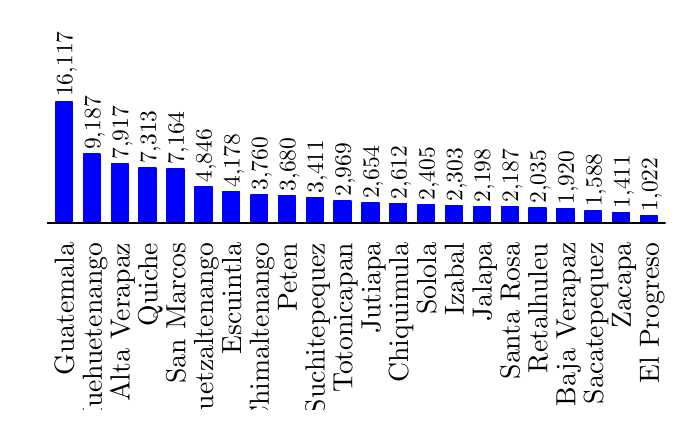
\begin{tikzpicture}[x=1pt,y=1pt]  % Created by tikzDevice version 0.7.0 on 2015-04-16 17:46:46
% !TEX encoding = UTF-8 Unicode
\definecolor[named]{fillColor}{rgb}{1.00,1.00,1.00}
\path[use as bounding box,fill=fillColor,fill opacity=0.00] (0,0) rectangle (230.54,138.04);
\begin{scope}
\path[clip] (  0.00,  0.00) rectangle (230.54,138.04);
\definecolor[named]{drawColor}{rgb}{1.00,1.00,1.00}

\path[draw=drawColor,line width= 0.6pt,line join=round,line cap=round] (  0.00,  0.00) rectangle (230.54,138.04);
\end{scope}
\begin{scope}
\path[clip] (  0.00,  0.00) rectangle (230.54,138.04);

\path[] (  7.11, 67.45) rectangle (230.54,111.19);

\path[] ( 13.15, 67.45) --
	( 13.15,111.19);

\path[] ( 23.22, 67.45) --
	( 23.22,111.19);

\path[] ( 33.28, 67.45) --
	( 33.28,111.19);

\path[] ( 43.34, 67.45) --
	( 43.34,111.19);

\path[] ( 53.41, 67.45) --
	( 53.41,111.19);

\path[] ( 63.47, 67.45) --
	( 63.47,111.19);

\path[] ( 73.54, 67.45) --
	( 73.54,111.19);

\path[] ( 83.60, 67.45) --
	( 83.60,111.19);

\path[] ( 93.67, 67.45) --
	( 93.67,111.19);

\path[] (103.73, 67.45) --
	(103.73,111.19);

\path[] (113.80, 67.45) --
	(113.80,111.19);

\path[] (123.86, 67.45) --
	(123.86,111.19);

\path[] (133.92, 67.45) --
	(133.92,111.19);

\path[] (143.99, 67.45) --
	(143.99,111.19);

\path[] (154.05, 67.45) --
	(154.05,111.19);

\path[] (164.12, 67.45) --
	(164.12,111.19);

\path[] (174.18, 67.45) --
	(174.18,111.19);

\path[] (184.25, 67.45) --
	(184.25,111.19);

\path[] (194.31, 67.45) --
	(194.31,111.19);

\path[] (204.37, 67.45) --
	(204.37,111.19);

\path[] (214.44, 67.45) --
	(214.44,111.19);

\path[] (224.50, 67.45) --
	(224.50,111.19);
\definecolor[named]{drawColor}{rgb}{0.00,0.00,1.00}
\definecolor[named]{fillColor}{rgb}{0.00,0.00,1.00}

\path[draw=drawColor,line width= 0.6pt,line join=round,fill=fillColor] ( 10.13, 67.45) rectangle ( 16.17,111.19);

\path[draw=drawColor,line width= 0.6pt,line join=round,fill=fillColor] ( 20.20, 67.45) rectangle ( 26.24, 92.38);

\path[draw=drawColor,line width= 0.6pt,line join=round,fill=fillColor] ( 30.26, 67.45) rectangle ( 36.30, 88.94);

\path[draw=drawColor,line width= 0.6pt,line join=round,fill=fillColor] ( 40.33, 67.45) rectangle ( 46.36, 87.30);

\path[draw=drawColor,line width= 0.6pt,line join=round,fill=fillColor] ( 50.39, 67.45) rectangle ( 56.43, 86.89);

\path[draw=drawColor,line width= 0.6pt,line join=round,fill=fillColor] ( 60.45, 67.45) rectangle ( 66.49, 80.60);

\path[draw=drawColor,line width= 0.6pt,line join=round,fill=fillColor] ( 70.52, 67.45) rectangle ( 76.56, 78.79);

\path[draw=drawColor,line width= 0.6pt,line join=round,fill=fillColor] ( 80.58, 67.45) rectangle ( 86.62, 77.66);

\path[draw=drawColor,line width= 0.6pt,line join=round,fill=fillColor] ( 90.65, 67.45) rectangle ( 96.69, 77.44);

\path[draw=drawColor,line width= 0.6pt,line join=round,fill=fillColor] (100.71, 67.45) rectangle (106.75, 76.71);

\path[draw=drawColor,line width= 0.6pt,line join=round,fill=fillColor] (110.78, 67.45) rectangle (116.81, 75.51);

\path[draw=drawColor,line width= 0.6pt,line join=round,fill=fillColor] (120.84, 67.45) rectangle (126.88, 74.65);

\path[draw=drawColor,line width= 0.6pt,line join=round,fill=fillColor] (130.90, 67.45) rectangle (136.94, 74.54);

\path[draw=drawColor,line width= 0.6pt,line join=round,fill=fillColor] (140.97, 67.45) rectangle (147.01, 73.98);

\path[draw=drawColor,line width= 0.6pt,line join=round,fill=fillColor] (151.03, 67.45) rectangle (157.07, 73.70);

\path[draw=drawColor,line width= 0.6pt,line join=round,fill=fillColor] (161.10, 67.45) rectangle (167.14, 73.42);

\path[draw=drawColor,line width= 0.6pt,line join=round,fill=fillColor] (171.16, 67.45) rectangle (177.20, 73.39);

\path[draw=drawColor,line width= 0.6pt,line join=round,fill=fillColor] (181.23, 67.45) rectangle (187.26, 72.97);

\path[draw=drawColor,line width= 0.6pt,line join=round,fill=fillColor] (191.29, 67.45) rectangle (197.33, 72.66);

\path[draw=drawColor,line width= 0.6pt,line join=round,fill=fillColor] (201.35, 67.45) rectangle (207.39, 71.76);

\path[draw=drawColor,line width= 0.6pt,line join=round,fill=fillColor] (211.42, 67.45) rectangle (217.46, 71.28);

\path[draw=drawColor,line width= 0.6pt,line join=round,fill=fillColor] (221.48, 67.45) rectangle (227.52, 70.22);
\definecolor[named]{drawColor}{rgb}{0.00,0.00,0.00}
\definecolor[named]{fillColor}{rgb}{0.00,0.00,0.00}

\path[draw=drawColor,line width= 0.6pt,line join=round,fill=fillColor] (  7.11, 67.45) -- (230.54, 67.45);

\node[text=drawColor,rotate= 90.00,anchor=base west,inner sep=0pt, outer sep=0pt, scale=  0.85] at ( 16.19,113.07) {16,117};

\node[text=drawColor,rotate= 90.00,anchor=base west,inner sep=0pt, outer sep=0pt, scale=  0.85] at ( 26.25, 93.92) {9,187};

\node[text=drawColor,rotate= 90.00,anchor=base west,inner sep=0pt, outer sep=0pt, scale=  0.85] at ( 36.32, 90.47) {7,917};

\node[text=drawColor,rotate= 90.00,anchor=base west,inner sep=0pt, outer sep=0pt, scale=  0.85] at ( 46.38, 88.83) {7,313};

\node[text=drawColor,rotate= 90.00,anchor=base west,inner sep=0pt, outer sep=0pt, scale=  0.85] at ( 56.44, 88.43) {7,164};

\node[text=drawColor,rotate= 90.00,anchor=base west,inner sep=0pt, outer sep=0pt, scale=  0.85] at ( 66.51, 82.14) {4,846};

\node[text=drawColor,rotate= 90.00,anchor=base west,inner sep=0pt, outer sep=0pt, scale=  0.85] at ( 76.57, 80.33) {4,178};

\node[text=drawColor,rotate= 90.00,anchor=base west,inner sep=0pt, outer sep=0pt, scale=  0.85] at ( 86.64, 79.19) {3,760};

\node[text=drawColor,rotate= 90.00,anchor=base west,inner sep=0pt, outer sep=0pt, scale=  0.85] at ( 96.70, 78.97) {3,680};

\node[text=drawColor,rotate= 90.00,anchor=base west,inner sep=0pt, outer sep=0pt, scale=  0.85] at (106.77, 78.24) {3,411};

\node[text=drawColor,rotate= 90.00,anchor=base west,inner sep=0pt, outer sep=0pt, scale=  0.85] at (116.83, 77.04) {2,969};

\node[text=drawColor,rotate= 90.00,anchor=base west,inner sep=0pt, outer sep=0pt, scale=  0.85] at (126.89, 76.19) {2,654};

\node[text=drawColor,rotate= 90.00,anchor=base west,inner sep=0pt, outer sep=0pt, scale=  0.85] at (136.96, 76.08) {2,612};

\node[text=drawColor,rotate= 90.00,anchor=base west,inner sep=0pt, outer sep=0pt, scale=  0.85] at (147.02, 75.51) {2,405};

\node[text=drawColor,rotate= 90.00,anchor=base west,inner sep=0pt, outer sep=0pt, scale=  0.85] at (157.09, 75.24) {2,303};

\node[text=drawColor,rotate= 90.00,anchor=base west,inner sep=0pt, outer sep=0pt, scale=  0.85] at (167.15, 74.95) {2,198};

\node[text=drawColor,rotate= 90.00,anchor=base west,inner sep=0pt, outer sep=0pt, scale=  0.85] at (177.22, 74.92) {2,187};

\node[text=drawColor,rotate= 90.00,anchor=base west,inner sep=0pt, outer sep=0pt, scale=  0.85] at (187.28, 74.51) {2,035};

\node[text=drawColor,rotate= 90.00,anchor=base west,inner sep=0pt, outer sep=0pt, scale=  0.85] at (197.35, 74.20) {1,920};

\node[text=drawColor,rotate= 90.00,anchor=base west,inner sep=0pt, outer sep=0pt, scale=  0.85] at (207.41, 73.30) {1,588};

\node[text=drawColor,rotate= 90.00,anchor=base west,inner sep=0pt, outer sep=0pt, scale=  0.85] at (217.47, 72.82) {1,411};

\node[text=drawColor,rotate= 90.00,anchor=base west,inner sep=0pt, outer sep=0pt, scale=  0.85] at (227.54, 71.76) {1,022};
\end{scope}
\begin{scope}
\path[clip] (  0.00,  0.00) rectangle (230.54,138.04);

\path[] (  7.11, 67.45) --
	(  7.11,111.19);
\end{scope}
\begin{scope}
\path[clip] (  0.00,  0.00) rectangle (230.54,138.04);

\path[] (  7.11, 67.45) --
	(230.54, 67.45);
\end{scope}
\begin{scope}
\path[clip] (  0.00,  0.00) rectangle (230.54,138.04);

\path[] ( 13.15, 63.18) --
	( 13.15, 67.45);

\path[] ( 23.22, 63.18) --
	( 23.22, 67.45);

\path[] ( 33.28, 63.18) --
	( 33.28, 67.45);

\path[] ( 43.34, 63.18) --
	( 43.34, 67.45);

\path[] ( 53.41, 63.18) --
	( 53.41, 67.45);

\path[] ( 63.47, 63.18) --
	( 63.47, 67.45);

\path[] ( 73.54, 63.18) --
	( 73.54, 67.45);

\path[] ( 83.60, 63.18) --
	( 83.60, 67.45);

\path[] ( 93.67, 63.18) --
	( 93.67, 67.45);

\path[] (103.73, 63.18) --
	(103.73, 67.45);

\path[] (113.80, 63.18) --
	(113.80, 67.45);

\path[] (123.86, 63.18) --
	(123.86, 67.45);

\path[] (133.92, 63.18) --
	(133.92, 67.45);

\path[] (143.99, 63.18) --
	(143.99, 67.45);

\path[] (154.05, 63.18) --
	(154.05, 67.45);

\path[] (164.12, 63.18) --
	(164.12, 67.45);

\path[] (174.18, 63.18) --
	(174.18, 67.45);

\path[] (184.25, 63.18) --
	(184.25, 67.45);

\path[] (194.31, 63.18) --
	(194.31, 67.45);

\path[] (204.37, 63.18) --
	(204.37, 67.45);

\path[] (214.44, 63.18) --
	(214.44, 67.45);

\path[] (224.50, 63.18) --
	(224.50, 67.45);
\end{scope}
\begin{scope}
\path[clip] (  0.00,  0.00) rectangle (230.54,138.04);
\definecolor[named]{drawColor}{rgb}{0.00,0.00,0.00}

\node[text=drawColor,rotate= 90.00,anchor=base east,inner sep=0pt, outer sep=0pt, scale=  1.00] at ( 16.72, 60.34) {Guatemala};

\node[text=drawColor,rotate= 90.00,anchor=base east,inner sep=0pt, outer sep=0pt, scale=  1.00] at ( 26.79, 60.34) {Huehuetenango};

\node[text=drawColor,rotate= 90.00,anchor=base east,inner sep=0pt, outer sep=0pt, scale=  1.00] at ( 36.85, 60.34) {Alta Verapaz};

\node[text=drawColor,rotate= 90.00,anchor=base east,inner sep=0pt, outer sep=0pt, scale=  1.00] at ( 46.91, 60.34) {Quiche};

\node[text=drawColor,rotate= 90.00,anchor=base east,inner sep=0pt, outer sep=0pt, scale=  1.00] at ( 56.98, 60.34) {San Marcos};

\node[text=drawColor,rotate= 90.00,anchor=base east,inner sep=0pt, outer sep=0pt, scale=  1.00] at ( 67.04, 60.34) {Quetzaltenango};

\node[text=drawColor,rotate= 90.00,anchor=base east,inner sep=0pt, outer sep=0pt, scale=  1.00] at ( 77.11, 60.34) {Escuintla};

\node[text=drawColor,rotate= 90.00,anchor=base east,inner sep=0pt, outer sep=0pt, scale=  1.00] at ( 87.17, 60.34) {Chimaltenango};

\node[text=drawColor,rotate= 90.00,anchor=base east,inner sep=0pt, outer sep=0pt, scale=  1.00] at ( 97.24, 60.34) {Peten};

\node[text=drawColor,rotate= 90.00,anchor=base east,inner sep=0pt, outer sep=0pt, scale=  1.00] at (107.30, 60.34) {Suchitepequez};

\node[text=drawColor,rotate= 90.00,anchor=base east,inner sep=0pt, outer sep=0pt, scale=  1.00] at (117.36, 60.34) {Totonicapan};

\node[text=drawColor,rotate= 90.00,anchor=base east,inner sep=0pt, outer sep=0pt, scale=  1.00] at (127.43, 60.34) {Jutiapa};

\node[text=drawColor,rotate= 90.00,anchor=base east,inner sep=0pt, outer sep=0pt, scale=  1.00] at (137.49, 60.34) {Chiquimula};

\node[text=drawColor,rotate= 90.00,anchor=base east,inner sep=0pt, outer sep=0pt, scale=  1.00] at (147.56, 60.34) {Solola};

\node[text=drawColor,rotate= 90.00,anchor=base east,inner sep=0pt, outer sep=0pt, scale=  1.00] at (157.62, 60.34) {Izabal};

\node[text=drawColor,rotate= 90.00,anchor=base east,inner sep=0pt, outer sep=0pt, scale=  1.00] at (167.69, 60.34) {Jalapa};

\node[text=drawColor,rotate= 90.00,anchor=base east,inner sep=0pt, outer sep=0pt, scale=  1.00] at (177.75, 60.34) {Santa Rosa};

\node[text=drawColor,rotate= 90.00,anchor=base east,inner sep=0pt, outer sep=0pt, scale=  1.00] at (187.81, 60.34) {Retalhuleu};

\node[text=drawColor,rotate= 90.00,anchor=base east,inner sep=0pt, outer sep=0pt, scale=  1.00] at (197.88, 60.34) {Baja Verapaz};

\node[text=drawColor,rotate= 90.00,anchor=base east,inner sep=0pt, outer sep=0pt, scale=  1.00] at (207.94, 60.34) {Sacatepequez};

\node[text=drawColor,rotate= 90.00,anchor=base east,inner sep=0pt, outer sep=0pt, scale=  1.00] at (218.01, 60.34) {Zacapa};

\node[text=drawColor,rotate= 90.00,anchor=base east,inner sep=0pt, outer sep=0pt, scale=  1.00] at (228.07, 60.34) {El Progreso};
\end{scope}
  \end{tikzpicture}}{Instituto Nacional de Estadística, con datos de Enei II-2014}

\cajita{Alfabetismo por edad}{Según la desagregación de la población en edad de trabajar por grandes grupos de edad, el 93\% de la población joven (comprendidos entre los 15 y 29 años) sabe leer y escribir, siendo este el grupo que presenta la mayor tasa de alfabetismo. Los adultos entre los 30 y 54 años presentan una tasa de alfabetismo del 78.4\%.}{Tasa de alfabetismo en personas mayores de 14 años\\ por grupo etario}{República de Guatemala, año 2014, en porcentaje}{\ \\[0mm]\begin{tikzpicture}[x=1pt,y=1pt]  % Created by tikzDevice version 0.10.1 on 2016-02-29 12:41:07
% !TEX encoding = UTF-8 Unicode
\definecolor{fillColor}{RGB}{255,255,255}
\path[use as bounding box,fill=fillColor,fill opacity=0.00] (0,0) rectangle (289.08,198.74);
\begin{scope}
\path[clip] ( 30.54,  0.00) rectangle (258.54,198.74);

\path[] ( 30.54,  0.00) rectangle (258.54,198.74);
\end{scope}
\begin{scope}
\path[clip] (  0.00,  0.00) rectangle (289.08,198.74);

\path[] (  7.11,  4.95) rectangle (200.91,198.74);

\path[] (104.01,101.85) --
	(171.12, 46.15);

\path[] (104.01,101.85) --
	( 36.90,157.54);

\path[] (104.01,101.85) --
	(159.70,168.95);

\path[] (104.01,101.85) --
	(171.12, 46.15);

\path[] (104.01,101.85) --
	( 48.32, 34.74);

\path[] (104.01,101.85) --
	( 36.90,157.54);

\path[] (104.01,101.85) --
	(104.01,101.85) --
	(104.01,101.85) --
	(104.01,101.85) --
	(104.01,101.85) --
	(104.01,101.85) --
	(104.01,101.85) --
	(104.01,101.85) --
	(104.01,101.85) --
	(104.01,101.85) --
	(104.01,101.85) --
	(104.01,101.85) --
	(104.01,101.85) --
	(104.01,101.85) --
	(104.01,101.85) --
	(104.01,101.85) --
	(104.01,101.85) --
	(104.01,101.85) --
	(104.01,101.85) --
	(104.01,101.85) --
	(104.01,101.85) --
	(104.01,101.85) --
	(104.01,101.85) --
	(104.01,101.85) --
	(104.01,101.85) --
	(104.01,101.85) --
	(104.01,101.85) --
	(104.01,101.85) --
	(104.01,101.85) --
	(104.01,101.85) --
	(104.01,101.85) --
	(104.01,101.85) --
	(104.01,101.85) --
	(104.01,101.85) --
	(104.01,101.85) --
	(104.01,101.85) --
	(104.01,101.85) --
	(104.01,101.85) --
	(104.01,101.85) --
	(104.01,101.85) --
	(104.01,101.85) --
	(104.01,101.85) --
	(104.01,101.85) --
	(104.01,101.85) --
	(104.01,101.85) --
	(104.01,101.85) --
	(104.01,101.85) --
	(104.01,101.85) --
	(104.01,101.85) --
	(104.01,101.85) --
	(104.01,101.85) --
	(104.01,101.85) --
	(104.01,101.85) --
	(104.01,101.85) --
	(104.01,101.85) --
	(104.01,101.85) --
	(104.01,101.85) --
	(104.01,101.85) --
	(104.01,101.85) --
	(104.01,101.85) --
	(104.01,101.85) --
	(104.01,101.85) --
	(104.01,101.85) --
	(104.01,101.85) --
	(104.01,101.85) --
	(104.01,101.85) --
	(104.01,101.85) --
	(104.01,101.85) --
	(104.01,101.85) --
	(104.01,101.85) --
	(104.01,101.85) --
	(104.01,101.85) --
	(104.01,101.85) --
	(104.01,101.85) --
	(104.01,101.85) --
	(104.01,101.85) --
	(104.01,101.85) --
	(104.01,101.85) --
	(104.01,101.85) --
	(104.01,101.85) --
	(104.01,101.85) --
	(104.01,101.85) --
	(104.01,101.85) --
	(104.01,101.85) --
	(104.01,101.85) --
	(104.01,101.85) --
	(104.01,101.85) --
	(104.01,101.85) --
	(104.01,101.85) --
	(104.01,101.85) --
	(104.01,101.85) --
	(104.01,101.85) --
	(104.01,101.85) --
	(104.01,101.85) --
	(104.01,101.85) --
	(104.01,101.85) --
	(104.01,101.85) --
	(104.01,101.85) --
	(104.01,101.85) --
	(104.01,101.85);

\path[] (104.01,121.23) --
	(105.24,121.19) --
	(106.46,121.07) --
	(107.68,120.88) --
	(108.88,120.60) --
	(110.06,120.26) --
	(111.21,119.84) --
	(112.34,119.34) --
	(113.43,118.78) --
	(114.49,118.15) --
	(115.50,117.45) --
	(116.47,116.69) --
	(117.38,115.87) --
	(118.25,115.00) --
	(119.05,114.07) --
	(119.80,113.09) --
	(120.48,112.06) --
	(121.09,111.00) --
	(121.64,109.90) --
	(122.11,108.76) --
	(122.51,107.60) --
	(122.84,106.42) --
	(123.09,105.21) --
	(123.27,103.99) --
	(123.37,102.77) --
	(123.39,101.54) --
	(123.33,100.31) --
	(123.19, 99.09) --
	(122.98, 97.88) --
	(122.69, 96.68) --
	(122.32, 95.51) --
	(121.88, 94.36) --
	(121.37, 93.24) --
	(120.79, 92.16) --
	(120.14, 91.11) --
	(119.43, 90.11) --
	(118.66, 89.16) --
	(117.82, 88.25) --
	(116.93, 87.40) --
	(115.99, 86.61) --
	(115.00, 85.88) --
	(113.96, 85.22) --
	(112.89, 84.62) --
	(111.78, 84.09) --
	(110.64, 83.64) --
	(109.47, 83.25) --
	(108.28, 82.94) --
	(107.07, 82.71) --
	(105.85, 82.55) --
	(104.62, 82.48) --
	(103.39, 82.48) --
	(102.17, 82.55) --
	(100.95, 82.71) --
	( 99.74, 82.94) --
	( 98.55, 83.25) --
	( 97.38, 83.64) --
	( 96.24, 84.09) --
	( 95.13, 84.62) --
	( 94.05, 85.22) --
	( 93.02, 85.88) --
	( 92.03, 86.61) --
	( 91.09, 87.40) --
	( 90.20, 88.25) --
	( 89.36, 89.16) --
	( 88.59, 90.11) --
	( 87.87, 91.11) --
	( 87.23, 92.16) --
	( 86.65, 93.24) --
	( 86.13, 94.36) --
	( 85.70, 95.51) --
	( 85.33, 96.68) --
	( 85.04, 97.88) --
	( 84.83, 99.09) --
	( 84.69,100.31) --
	( 84.63,101.54) --
	( 84.65,102.77) --
	( 84.75,103.99) --
	( 84.92,105.21) --
	( 85.18,106.42) --
	( 85.50,107.60) --
	( 85.91,108.76) --
	( 86.38,109.90) --
	( 86.93,111.00) --
	( 87.54,112.06) --
	( 88.22,113.09) --
	( 88.97,114.07) --
	( 89.77,115.00) --
	( 90.64,115.87) --
	( 91.55,116.69) --
	( 92.52,117.45) --
	( 93.53,118.15) --
	( 94.59,118.78) --
	( 95.68,119.34) --
	( 96.81,119.84) --
	( 97.96,120.26) --
	( 99.14,120.60) --
	(100.34,120.88) --
	(101.56,121.07) --
	(102.78,121.19) --
	(104.01,121.23);

\path[] (104.01,140.60) --
	(106.47,140.53) --
	(108.92,140.29) --
	(111.34,139.90) --
	(113.74,139.36) --
	(116.10,138.67) --
	(118.41,137.83) --
	(120.67,136.84) --
	(122.85,135.72) --
	(124.96,134.45) --
	(126.99,133.06) --
	(128.92,131.54) --
	(130.76,129.90) --
	(132.48,128.14) --
	(134.09,126.29) --
	(135.58,124.33) --
	(136.94,122.28) --
	(138.17,120.15) --
	(139.27,117.95) --
	(140.22,115.68) --
	(141.02,113.35) --
	(141.68,110.98) --
	(142.18,108.58) --
	(142.53,106.14) --
	(142.72,103.69) --
	(142.76,101.23) --
	(142.65, 98.77) --
	(142.37, 96.33) --
	(141.95, 93.91) --
	(141.37, 91.52) --
	(140.64, 89.17) --
	(139.76, 86.87) --
	(138.74, 84.63) --
	(137.58, 82.47) --
	(136.28, 80.38) --
	(134.85, 78.37) --
	(133.30, 76.46) --
	(131.63, 74.66) --
	(129.85, 72.96) --
	(127.97, 71.38) --
	(125.99, 69.92) --
	(123.92, 68.59) --
	(121.77, 67.40) --
	(119.55, 66.34) --
	(117.27, 65.43) --
	(114.93, 64.66) --
	(112.55, 64.04) --
	(110.13, 63.57) --
	(107.69, 63.26) --
	(105.24, 63.11) --
	(102.78, 63.11) --
	(100.33, 63.26) --
	( 97.89, 63.57) --
	( 95.47, 64.04) --
	( 93.09, 64.66) --
	( 90.75, 65.43) --
	( 88.47, 66.34) --
	( 86.25, 67.40) --
	( 84.10, 68.59) --
	( 82.03, 69.92) --
	( 80.05, 71.38) --
	( 78.17, 72.96) --
	( 76.39, 74.66) --
	( 74.72, 76.46) --
	( 73.17, 78.37) --
	( 71.74, 80.38) --
	( 70.44, 82.47) --
	( 69.28, 84.63) --
	( 68.26, 86.87) --
	( 67.38, 89.17) --
	( 66.65, 91.52) --
	( 66.07, 93.91) --
	( 65.65, 96.33) --
	( 65.37, 98.77) --
	( 65.26,101.23) --
	( 65.29,103.69) --
	( 65.49,106.14) --
	( 65.84,108.58) --
	( 66.34,110.98) --
	( 67.00,113.35) --
	( 67.80,115.68) --
	( 68.75,117.95) --
	( 69.85,120.15) --
	( 71.08,122.28) --
	( 72.44,124.33) --
	( 73.93,126.29) --
	( 75.54,128.14) --
	( 77.26,129.90) --
	( 79.10,131.54) --
	( 81.03,133.06) --
	( 83.06,134.45) --
	( 85.17,135.72) --
	( 87.35,136.84) --
	( 89.60,137.83) --
	( 91.92,138.67) --
	( 94.28,139.36) --
	( 96.67,139.90) --
	( 99.10,140.29) --
	(101.55,140.53) --
	(104.01,140.60);

\path[] (104.01,159.98) --
	(107.70,159.87) --
	(111.37,159.52) --
	(115.01,158.93) --
	(118.61,158.12) --
	(122.15,157.08) --
	(125.62,155.82) --
	(129.00,154.34) --
	(132.28,152.65) --
	(135.44,150.75) --
	(138.48,148.66) --
	(141.38,146.38) --
	(144.13,143.92) --
	(146.72,141.29) --
	(149.13,138.51) --
	(151.37,135.57) --
	(153.41,132.50) --
	(155.26,129.30) --
	(156.89,126.00) --
	(158.32,122.59) --
	(159.53,119.11) --
	(160.51,115.55) --
	(161.26,111.94) --
	(161.79,108.29) --
	(162.08,104.61) --
	(162.14,100.92) --
	(161.96, 97.24) --
	(161.56, 93.57) --
	(160.91, 89.94) --
	(160.05, 86.35) --
	(158.95, 82.83) --
	(157.63, 79.39) --
	(156.10, 76.03) --
	(154.36, 72.78) --
	(152.41, 69.64) --
	(150.27, 66.64) --
	(147.95, 63.77) --
	(145.44, 61.06) --
	(142.77, 58.52) --
	(139.95, 56.15) --
	(136.98, 53.96) --
	(133.87, 51.97) --
	(130.65, 50.17) --
	(127.32, 48.59) --
	(123.89, 47.21) --
	(120.39, 46.06) --
	(116.82, 45.14) --
	(113.20, 44.44) --
	(109.54, 43.97) --
	(105.85, 43.74) --
	(102.16, 43.74) --
	( 98.48, 43.97) --
	( 94.82, 44.44) --
	( 91.20, 45.14) --
	( 87.63, 46.06) --
	( 84.13, 47.21) --
	( 80.70, 48.59) --
	( 77.37, 50.17) --
	( 74.15, 51.97) --
	( 71.04, 53.96) --
	( 68.07, 56.15) --
	( 65.25, 58.52) --
	( 62.58, 61.06) --
	( 60.07, 63.77) --
	( 57.75, 66.64) --
	( 55.61, 69.64) --
	( 53.66, 72.78) --
	( 51.92, 76.03) --
	( 50.39, 79.39) --
	( 49.07, 82.83) --
	( 47.97, 86.35) --
	( 47.10, 89.94) --
	( 46.46, 93.57) --
	( 46.05, 97.24) --
	( 45.88,100.92) --
	( 45.94,104.61) --
	( 46.23,108.29) --
	( 46.75,111.94) --
	( 47.51,115.55) --
	( 48.49,119.11) --
	( 49.70,122.59) --
	( 51.13,126.00) --
	( 52.76,129.30) --
	( 54.61,132.50) --
	( 56.65,135.57) --
	( 58.89,138.51) --
	( 61.30,141.29) --
	( 63.89,143.92) --
	( 66.64,146.38) --
	( 69.54,148.66) --
	( 72.58,150.75) --
	( 75.74,152.65) --
	( 79.02,154.34) --
	( 82.40,155.82) --
	( 85.87,157.08) --
	( 89.41,158.12) --
	( 93.01,158.93) --
	( 96.65,159.52) --
	(100.32,159.87) --
	(104.01,159.98);

\path[] (104.01,179.36) --
	(108.93,179.21) --
	(113.82,178.74) --
	(118.68,177.96) --
	(123.48,176.88) --
	(128.20,175.49) --
	(132.82,173.81) --
	(137.33,171.84) --
	(141.70,169.58) --
	(145.92,167.06) --
	(149.97,164.27) --
	(153.84,161.23) --
	(157.50,157.95) --
	(160.95,154.44) --
	(164.17,150.72) --
	(167.15,146.81) --
	(169.88,142.72) --
	(172.34,138.46) --
	(174.52,134.05) --
	(176.42,129.51) --
	(178.03,124.86) --
	(179.34,120.12) --
	(180.35,115.31) --
	(181.05,110.44) --
	(181.44,105.53) --
	(181.52,100.62) --
	(181.28, 95.70) --
	(180.74, 90.81) --
	(179.88, 85.97) --
	(178.72, 81.19) --
	(177.26, 76.49) --
	(175.51, 71.90) --
	(173.46, 67.42) --
	(171.14, 63.09) --
	(168.55, 58.91) --
	(165.69, 54.90) --
	(162.59, 51.08) --
	(159.26, 47.47) --
	(155.70, 44.08) --
	(151.93, 40.91) --
	(147.97, 38.00) --
	(143.83, 35.34) --
	(139.53, 32.95) --
	(135.09, 30.83) --
	(130.52, 29.00) --
	(125.85, 27.47) --
	(121.09, 26.23) --
	(116.26, 25.30) --
	(111.38, 24.68) --
	(106.47, 24.37) --
	(101.55, 24.37) --
	( 96.64, 24.68) --
	( 91.76, 25.30) --
	( 86.93, 26.23) --
	( 82.17, 27.47) --
	( 77.50, 29.00) --
	( 72.93, 30.83) --
	( 68.49, 32.95) --
	( 64.19, 35.34) --
	( 60.05, 38.00) --
	( 56.09, 40.91) --
	( 52.32, 44.08) --
	( 48.76, 47.47) --
	( 45.43, 51.08) --
	( 42.32, 54.90) --
	( 39.47, 58.91) --
	( 36.88, 63.09) --
	( 34.55, 67.42) --
	( 32.51, 71.90) --
	( 30.76, 76.49) --
	( 29.30, 81.19) --
	( 28.14, 85.97) --
	( 27.28, 90.81) --
	( 26.74, 95.70) --
	( 26.50,100.62) --
	( 26.58,105.53) --
	( 26.97,110.44) --
	( 27.67,115.31) --
	( 28.68,120.12) --
	( 29.99,124.86) --
	( 31.60,129.51) --
	( 33.50,134.05) --
	( 35.68,138.46) --
	( 38.14,142.72) --
	( 40.87,146.81) --
	( 43.84,150.72) --
	( 47.07,154.44) --
	( 50.52,157.95) --
	( 54.18,161.23) --
	( 58.05,164.27) --
	( 62.10,167.06) --
	( 66.32,169.58) --
	( 70.69,171.84) --
	( 75.20,173.81) --
	( 79.82,175.49) --
	( 84.54,176.88) --
	( 89.34,177.96) --
	( 94.20,178.74) --
	( 99.09,179.21) --
	(104.01,179.36);

\path[] (104.01,189.05) --
	(109.54,188.88) --
	(115.05,188.35) --
	(120.51,187.48) --
	(125.91,186.26) --
	(131.22,184.70) --
	(136.42,182.81) --
	(141.49,180.59) --
	(146.41,178.05) --
	(151.16,175.21) --
	(155.71,172.07) --
	(160.06,168.65) --
	(164.19,164.96) --
	(168.07,161.02) --
	(171.69,156.83) --
	(175.05,152.43) --
	(178.11,147.82) --
	(180.88,143.03) --
	(183.34,138.07) --
	(185.47,132.97) --
	(187.28,127.74) --
	(188.76,122.41) --
	(189.89,116.99) --
	(190.68,111.51) --
	(191.12,106.00) --
	(191.21,100.46) --
	(190.94, 94.94) --
	(190.33, 89.44) --
	(189.37, 83.99) --
	(188.06, 78.61) --
	(186.42, 73.32) --
	(184.44, 68.15) --
	(182.15, 63.12) --
	(179.53, 58.24) --
	(176.62, 53.54) --
	(173.41, 49.03) --
	(169.92, 44.74) --
	(166.16, 40.67) --
	(162.16, 36.85) --
	(157.92, 33.30) --
	(153.46, 30.02) --
	(148.81, 27.02) --
	(143.97, 24.33) --
	(138.97, 21.96) --
	(133.84, 19.90) --
	(128.58, 18.17) --
	(123.22, 16.78) --
	(117.79, 15.74) --
	(112.30, 15.03) --
	(106.78, 14.68) --
	(101.24, 14.68) --
	( 95.72, 15.03) --
	( 90.23, 15.74) --
	( 84.80, 16.78) --
	( 79.44, 18.17) --
	( 74.18, 19.90) --
	( 69.05, 21.96) --
	( 64.05, 24.33) --
	( 59.21, 27.02) --
	( 54.56, 30.02) --
	( 50.10, 33.30) --
	( 45.86, 36.85) --
	( 41.86, 40.67) --
	( 38.10, 44.74) --
	( 34.61, 49.03) --
	( 31.40, 53.54) --
	( 28.49, 58.24) --
	( 25.87, 63.12) --
	( 23.57, 68.15) --
	( 21.60, 73.32) --
	( 19.96, 78.61) --
	( 18.65, 83.99) --
	( 17.69, 89.44) --
	( 17.08, 94.94) --
	( 16.81,100.46) --
	( 16.90,106.00) --
	( 17.34,111.51) --
	( 18.13,116.99) --
	( 19.26,122.41) --
	( 20.74,127.74) --
	( 22.55,132.97) --
	( 24.68,138.07) --
	( 27.14,143.03) --
	( 29.91,147.82) --
	( 32.97,152.43) --
	( 36.32,156.83) --
	( 39.95,161.02) --
	( 43.83,164.96) --
	( 47.95,168.65) --
	( 52.30,172.07) --
	( 56.86,175.21) --
	( 61.61,178.05) --
	( 66.53,180.59) --
	( 71.60,182.81) --
	( 76.80,184.70) --
	( 82.11,186.26) --
	( 87.51,187.48) --
	( 92.97,188.35) --
	( 98.48,188.88) --
	(104.01,189.05);
\definecolor{drawColor}{RGB}{255,255,255}
\definecolor{fillColor}{RGB}{0,0,255}

\path[draw=drawColor,line width= 0.6pt,line join=round,line cap=round,fill=fillColor] ( 65.91, 94.70) --
	( 63.19, 94.19) --
	( 60.47, 93.68) --
	( 57.75, 93.17) --
	( 55.03, 92.66) --
	( 52.31, 92.15) --
	( 49.59, 91.64) --
	( 46.87, 91.13) --
	( 44.15, 90.62) --
	( 41.43, 90.11) --
	( 38.70, 89.60) --
	( 35.98, 89.09) --
	( 33.26, 88.58) --
	( 30.54, 88.07) --
	( 27.82, 87.56) --
	( 28.35, 84.98) --
	( 28.97, 82.41) --
	( 29.67, 79.87) --
	( 30.46, 77.35) --
	( 31.34, 74.86) --
	( 32.30, 72.40) --
	( 33.34, 69.98) --
	( 34.47, 67.60) --
	( 35.68, 65.25) --
	( 36.96, 62.94) --
	( 38.32, 60.68) --
	( 39.76, 58.47) --
	( 41.28, 56.31) --
	( 42.86, 54.20) --
	( 44.52, 52.15) --
	( 46.24, 50.15) --
	( 48.04, 48.22) --
	( 49.89, 46.34) --
	( 51.81, 44.54) --
	( 53.79, 42.79) --
	( 55.83, 41.12) --
	( 57.93, 39.51) --
	( 60.08, 37.98) --
	( 62.27, 36.52) --
	( 64.52, 35.14) --
	( 66.82, 33.84) --
	( 69.15, 32.61) --
	( 71.53, 31.46) --
	( 73.94, 30.40) --
	( 76.39, 29.42) --
	( 78.87, 28.52) --
	( 81.38, 27.71) --
	( 83.92, 26.98) --
	( 86.48, 26.34) --
	( 89.06, 25.79) --
	( 91.65, 25.32) --
	( 94.27, 24.94) --
	( 96.89, 24.66) --
	( 99.52, 24.46) --
	(102.16, 24.35) --
	(104.79, 24.33) --
	(107.43, 24.40) --
	(110.06, 24.57) --
	(112.69, 24.82) --
	(115.31, 25.16) --
	(117.91, 25.59) --
	(120.50, 26.10) --
	(123.07, 26.71) --
	(125.61, 27.40) --
	(128.13, 28.18) --
	(130.63, 29.04) --
	(133.09, 29.99) --
	(135.52, 31.02) --
	(137.91, 32.13) --
	(140.26, 33.33) --
	(142.57, 34.60) --
	(144.84, 35.95) --
	(147.06, 37.38) --
	(149.23, 38.88) --
	(151.34, 40.46) --
	(153.40, 42.10) --
	(155.41, 43.82) --
	(157.35, 45.60) --
	(159.24, 47.45) --
	(161.06, 49.36) --
	(162.81, 51.33) --
	(164.49, 53.36) --
	(166.11, 55.45) --
	(167.65, 57.59) --
	(169.12, 59.78) --
	(170.51, 62.02) --
	(171.83, 64.31) --
	(173.07, 66.64) --
	(174.23, 69.01) --
	(175.30, 71.42) --
	(176.30, 73.86) --
	(177.21, 76.34) --
	(178.03, 78.84) --
	(178.77, 81.38) --
	(179.43, 83.93) --
	(179.99, 86.51) --
	(180.47, 89.10) --
	(180.86, 91.71) --
	(181.16, 94.33) --
	(181.37, 96.96) --
	(181.49, 99.60) --
	(181.53,102.24) --
	(181.47,104.88) --
	(181.32,107.51) --
	(181.08,110.14) --
	(180.75,112.76) --
	(180.34,115.36) --
	(179.84,117.95) --
	(179.24,120.52) --
	(178.56,123.07) --
	(177.80,125.60) --
	(176.95,128.09) --
	(176.01,130.56) --
	(174.99,132.99) --
	(173.89,135.39) --
	(172.71,137.75) --
	(171.45,140.07) --
	(170.11,142.34) --
	(168.69,144.57) --
	(167.20,146.74) --
	(165.64,148.87) --
	(164.00,150.94) --
	(162.29,152.95) --
	(160.52,154.91) --
	(158.68,156.80) --
	(156.78,158.63) --
	(154.82,160.39) --
	(152.80,162.08) --
	(150.72,163.71) --
	(148.59,165.26) --
	(146.40,166.74) --
	(144.17,168.15) --
	(141.89,169.48) --
	(139.57,170.73) --
	(137.20,171.90) --
	(134.80,172.99) --
	(132.36,173.99) --
	(129.89,174.92) --
	(127.39,175.75) --
	(124.86,176.51) --
	(122.30,177.17) --
	(119.73,177.75) --
	(117.14,178.24) --
	(114.53,178.65) --
	(111.91,178.96) --
	(109.28,179.18) --
	(106.65,179.32) --
	(104.01,179.36) --
	(104.01,176.59) --
	(104.01,173.83) --
	(104.01,171.06) --
	(104.01,168.29) --
	(104.01,165.52) --
	(104.01,162.75) --
	(104.01,159.98) --
	(104.01,157.22) --
	(104.01,154.45) --
	(104.01,151.68) --
	(104.01,148.91) --
	(104.01,146.14) --
	(104.01,143.37) --
	(104.01,140.60) --
	(106.67,140.51) --
	(109.31,140.24) --
	(111.93,139.79) --
	(114.51,139.16) --
	(117.04,138.35) --
	(119.51,137.37) --
	(121.91,136.22) --
	(124.23,134.91) --
	(126.44,133.45) --
	(128.56,131.84) --
	(130.56,130.09) --
	(132.43,128.20) --
	(134.17,126.19) --
	(135.77,124.07) --
	(137.21,121.84) --
	(138.51,119.51) --
	(139.64,117.11) --
	(140.60,114.63) --
	(141.39,112.09) --
	(142.00,109.51) --
	(142.44,106.89) --
	(142.69,104.24) --
	(142.77,101.58) --
	(142.66, 98.93) --
	(142.37, 96.28) --
	(141.90, 93.67) --
	(141.25, 91.09) --
	(140.42, 88.56) --
	(139.43, 86.10) --
	(138.26, 83.71) --
	(136.94, 81.41) --
	(135.46, 79.20) --
	(133.83, 77.09) --
	(132.07, 75.11) --
	(130.17, 73.25) --
	(128.15, 71.52) --
	(126.01, 69.94) --
	(123.77, 68.51) --
	(121.44, 67.23) --
	(119.03, 66.12) --
	(116.55, 65.17) --
	(114.00, 64.40) --
	(111.41, 63.80) --
	(108.79, 63.38) --
	(106.14, 63.15) --
	(103.48, 63.09) --
	(100.83, 63.22) --
	( 98.19, 63.53) --
	( 95.57, 64.02) --
	( 93.00, 64.68) --
	( 90.48, 65.53) --
	( 88.02, 66.54) --
	( 85.64, 67.72) --
	( 83.34, 69.06) --
	( 81.15, 70.55) --
	( 79.05, 72.19) --
	( 77.08, 73.97) --
	( 75.23, 75.88) --
	( 73.52, 77.91) --
	( 71.95, 80.06) --
	( 70.54, 82.31) --
	( 69.28, 84.65) --
	( 68.18, 87.07) --
	( 67.25, 89.56) --
	( 66.49, 92.11) --
	( 65.91, 94.70) --
	cycle;
\definecolor{fillColor}{RGB}{157,187,255}

\path[draw=drawColor,line width= 0.6pt,line join=round,line cap=round,fill=fillColor] (104.01,140.60) --
	(104.01,143.37) --
	(104.01,146.14) --
	(104.01,148.91) --
	(104.01,151.68) --
	(104.01,154.45) --
	(104.01,157.22) --
	(104.01,159.98) --
	(104.01,162.75) --
	(104.01,165.52) --
	(104.01,168.29) --
	(104.01,171.06) --
	(104.01,173.83) --
	(104.01,176.59) --
	(104.01,179.36) --
	(101.34,179.32) --
	( 98.68,179.18) --
	( 96.02,178.95) --
	( 93.37,178.63) --
	( 90.73,178.22) --
	( 88.11,177.71) --
	( 85.51,177.12) --
	( 82.92,176.44) --
	( 80.37,175.67) --
	( 77.84,174.81) --
	( 75.34,173.87) --
	( 72.88,172.84) --
	( 70.46,171.73) --
	( 68.07,170.53) --
	( 65.73,169.25) --
	( 63.43,167.89) --
	( 61.18,166.46) --
	( 58.98,164.94) --
	( 56.84,163.36) --
	( 54.75,161.70) --
	( 52.71,159.96) --
	( 50.74,158.16) --
	( 48.84,156.30) --
	( 46.99,154.36) --
	( 45.22,152.37) --
	( 43.52,150.32) --
	( 41.88,148.21) --
	( 40.32,146.04) --
	( 38.84,143.82) --
	( 37.43,141.55) --
	( 36.11,139.24) --
	( 34.86,136.88) --
	( 33.69,134.47) --
	( 32.61,132.03) --
	( 31.62,129.56) --
	( 30.70,127.05) --
	( 29.88,124.51) --
	( 29.14,121.95) --
	( 28.50,119.36) --
	( 27.94,116.75) --
	( 27.47,114.12) --
	( 27.09,111.48) --
	( 26.81,108.82) --
	( 26.61,106.16) --
	( 26.51,103.49) --
	( 26.50,100.82) --
	( 26.58, 98.16) --
	( 26.75, 95.49) --
	( 27.02, 92.84) --
	( 27.37, 90.19) --
	( 27.82, 87.56) --
	( 30.54, 88.07) --
	( 33.26, 88.58) --
	( 35.98, 89.09) --
	( 38.70, 89.60) --
	( 41.43, 90.11) --
	( 44.15, 90.62) --
	( 46.87, 91.13) --
	( 49.59, 91.64) --
	( 52.31, 92.15) --
	( 55.03, 92.66) --
	( 57.75, 93.17) --
	( 60.47, 93.68) --
	( 63.19, 94.19) --
	( 65.91, 94.70) --
	( 65.51, 97.39) --
	( 65.29,100.11) --
	( 65.26,102.83) --
	( 65.43,105.55) --
	( 65.78,108.25) --
	( 66.33,110.91) --
	( 67.06,113.54) --
	( 67.97,116.10) --
	( 69.06,118.60) --
	( 70.32,121.01) --
	( 71.75,123.32) --
	( 73.33,125.54) --
	( 75.07,127.63) --
	( 76.95,129.60) --
	( 78.97,131.43) --
	( 81.11,133.11) --
	( 83.36,134.64) --
	( 85.71,136.01) --
	( 88.15,137.21) --
	( 90.67,138.24) --
	( 93.26,139.08) --
	( 95.90,139.75) --
	( 98.58,140.22) --
	(101.29,140.51) --
	(104.01,140.60) --
	cycle;
\definecolor{drawColor}{RGB}{0,0,0}

\node[text=drawColor,anchor=base,inner sep=0pt, outer sep=0pt, scale=  1.00] at (171.12, 42.25) {72};

\node[text=drawColor,anchor=base,inner sep=0pt, outer sep=0pt, scale=  1.00] at ( 36.90,153.63) {28};

\path[] (  7.11,  4.95) rectangle (200.91,198.74);
\end{scope}
\begin{scope}
\path[clip] (  0.00,  0.00) rectangle (289.08,198.74);

\path[] (  7.11,  4.95) --
	(  7.11,198.74);
\end{scope}
\begin{scope}
\path[clip] (  0.00,  0.00) rectangle (289.08,198.74);

\path[] (  4.36,101.85) --
	(  7.11,101.85);

\path[] (  4.36,121.23) --
	(  7.11,121.23);

\path[] (  4.36,140.60) --
	(  7.11,140.60);

\path[] (  4.36,159.98) --
	(  7.11,159.98);

\path[] (  4.36,179.36) --
	(  7.11,179.36);
\end{scope}
\begin{scope}
\path[clip] (  0.00,  0.00) rectangle (289.08,198.74);

\path[] (  7.11,  4.95) --
	(200.91,  4.95);
\end{scope}
\begin{scope}
\path[clip] (  0.00,  0.00) rectangle (289.08,198.74);
\coordinate (rect) at (192.72,99.37);
\coordinate (desY) at (0,18.49);
\coordinate (desX) at (7.11,11.38);
\coordinate (mdesX) at (7.11,-11.38);
\definecolor[named]{ct1}{HTML}{
0000FF
}
\definecolor[named]{borde}{HTML}{
0000FF
}
\coordinate (t1) at ($(rect) + 0.5*(desX) + 0.5*(desY)$);
\coordinate (t2) at ($(rect)+0.5*(mdesX)-0.5*(desY)$);
\draw [color=ct1,fill=borde] ($(rect)+(desY)$) rectangle ($(rect)+(desX)$);
\definecolor[named]{ct2}{HTML}{
9DBBFF
}
\node [text width=
56.692913328
,right= 0.3cm of t1,scale = 0.9]{
No indígenas
};
\path [fill=ct2] ($(rect)-(desY)$) rectangle ($(rect)+(mdesX)$);
\node [text width=
56.692913328
,right= 0.3cm of t2,scale = 0.9]{
Indígenas
};
\end{scope}
  \end{tikzpicture}}{Instituto Nacional de Estadística, con datos de Enei II-2014}

\cajita{Alfabetismo por etnia}{Con la desagregación de la tasa de alfabetismo de las personas en edad de trabajar según su grupo étnico, se muestra que las personas no indígenas presentan la tasa mayor de alfabetismo (83.8\%) comparada con la de la población indígena (64.1\%) ,indica que la tasa de analfabetismo es 2.2 veces mayor en la población indígena.}{Tasa de alfabetismo en personas mayores\\ de 14 años por grupo étnico}{República de Guatemala, año 2014, en porcentaje}{\ \\[0mm]\begin{tikzpicture}[x=1pt,y=1pt]  % Created by tikzDevice version 0.7.0 on 2015-08-28 14:02:54
% !TEX encoding = UTF-8 Unicode
\definecolor[named]{fillColor}{rgb}{1.00,1.00,1.00}
\path[use as bounding box,fill=fillColor,fill opacity=0.00] (0,0) rectangle (289.08,198.74);
\begin{scope}
\path[clip] (  0.00,  0.00) rectangle (289.08,198.74);
\definecolor[named]{drawColor}{rgb}{1.00,1.00,1.00}

\path[draw=drawColor,line width= 0.6pt,line join=round,line cap=round] (  0.00,  0.00) rectangle (289.08,198.74);
\end{scope}
\begin{scope}
\path[clip] (  0.00,  0.00) rectangle (289.08,198.74);

\path[] (  7.11, 20.62) rectangle (289.08,172.85);

\path[] ( 59.98, 20.62) --
	( 59.98,172.85);

\path[] (148.10, 20.62) --
	(148.10,172.85);

\path[] (236.21, 20.62) --
	(236.21,172.85);
\definecolor[named]{drawColor}{rgb}{0.00,0.00,1.00}
\definecolor[named]{fillColor}{rgb}{0.00,0.00,1.00}

\path[draw=drawColor,line width= 0.6pt,line join=round,fill=fillColor] ( 26.06, 20.62) rectangle ( 54.25,169.47);
\definecolor[named]{drawColor}{rgb}{0.62,0.73,1.00}
\definecolor[named]{fillColor}{rgb}{0.62,0.73,1.00}

\path[draw=drawColor,line width= 0.6pt,line join=round,fill=fillColor] ( 65.71, 20.62) rectangle ( 93.91,172.85);
\definecolor[named]{drawColor}{rgb}{0.00,0.00,1.00}
\definecolor[named]{fillColor}{rgb}{0.00,0.00,1.00}

\path[draw=drawColor,line width= 0.6pt,line join=round,fill=fillColor] (114.17, 20.62) rectangle (142.37, 40.58);
\definecolor[named]{drawColor}{rgb}{0.62,0.73,1.00}
\definecolor[named]{fillColor}{rgb}{0.62,0.73,1.00}

\path[draw=drawColor,line width= 0.6pt,line join=round,fill=fillColor] (153.82, 20.62) rectangle (182.02, 37.20);
\definecolor[named]{drawColor}{rgb}{0.00,0.00,1.00}
\definecolor[named]{fillColor}{rgb}{0.00,0.00,1.00}

\path[draw=drawColor,line width= 0.6pt,line join=round,fill=fillColor] (202.29, 20.62) rectangle (230.48, 20.96);
\definecolor[named]{drawColor}{rgb}{0.62,0.73,1.00}
\definecolor[named]{fillColor}{rgb}{0.62,0.73,1.00}

\path[draw=drawColor,line width= 0.6pt,line join=round,fill=fillColor] (241.94, 20.62) rectangle (270.14, 20.79);
\definecolor[named]{drawColor}{rgb}{0.00,0.00,0.00}
\definecolor[named]{fillColor}{rgb}{0.00,0.00,0.00}

\path[draw=drawColor,line width= 0.6pt,line join=round,fill=fillColor] (  7.11, 20.62) -- (289.08, 20.62);

\node[text=drawColor,anchor=base,inner sep=0pt, outer sep=0pt, scale=  0.82] at ( 40.16,172.69) {88.0};

\node[text=drawColor,anchor=base,inner sep=0pt, outer sep=0pt, scale=  0.82] at ( 79.81,176.07) {90.0};

\node[text=drawColor,anchor=base,inner sep=0pt, outer sep=0pt, scale=  0.82] at (128.27, 43.80) {11.8};

\node[text=drawColor,anchor=base,inner sep=0pt, outer sep=0pt, scale=  0.82] at (167.92, 40.42) {9.8};

\node[text=drawColor,anchor=base,inner sep=0pt, outer sep=0pt, scale=  0.82] at (216.39, 24.18) {0.2};

\node[text=drawColor,anchor=base,inner sep=0pt, outer sep=0pt, scale=  0.82] at (256.04, 24.01) {0.1};
\end{scope}
\begin{scope}
\path[clip] (  0.00,  0.00) rectangle (289.08,198.74);

\path[] (  7.11, 20.62) --
	(  7.11,172.85);
\end{scope}
\begin{scope}
\path[clip] (  0.00,  0.00) rectangle (289.08,198.74);

\path[] (  7.11, 20.62) --
	(289.08, 20.62);
\end{scope}
\begin{scope}
\path[clip] (  0.00,  0.00) rectangle (289.08,198.74);

\path[] ( 59.98, 16.35) --
	( 59.98, 20.62);

\path[] (148.10, 16.35) --
	(148.10, 20.62);

\path[] (236.21, 16.35) --
	(236.21, 20.62);
\end{scope}
\begin{scope}
\path[clip] (  0.00,  0.00) rectangle (289.08,198.74);
\definecolor[named]{drawColor}{rgb}{0.00,0.00,0.00}

\node[text=drawColor,anchor=base,inner sep=0pt, outer sep=0pt, scale=  1.00] at ( 59.98,  5.69) {T\'ecnico y licenciatura};

\node[text=drawColor,anchor=base,inner sep=0pt, outer sep=0pt, scale=  1.00] at (148.10,  5.69) {Maestr\'ia};

\node[text=drawColor,anchor=base,inner sep=0pt, outer sep=0pt, scale=  1.00] at (236.21,  5.69) {Doctorado};
\end{scope}
\coordinate (apoyo) at (55.98,189.21);
\coordinate (longitudFicticia) at (7.11,9.53);
\coordinate (longitud) at (7.11,7.11);
\coordinate (desX) at (142.21,0);
\coordinate (desY) at (0,1.21);
\definecolor[named]{ct1}{HTML}{
0000FF
}
\definecolor[named]{ct2}{HTML}{
9DBBFF
}
\definecolor[named]{ctb1}{HTML}{
0000FF
}
\definecolor[named]{ctb2}{HTML}{
9DBBFF
}
\path [fill=none] (apoyo) rectangle ($(apoyo)+(longitudFicticia)$)
node [xshift=0.3cm,inner sep=0pt, outer sep=0pt,midway,right,scale = 0.9]{Hombre};
\draw [color = ctb1,fill=ct1] ( $(apoyo)  + (desY) $) rectangle ($(apoyo)+ (desY) +(longitud)$);
\path [fill=none] ($(apoyo)+(desX)$) rectangle ($(apoyo)+(desX)+(longitudFicticia)$)
node [xshift=0.3cm,inner sep=0pt, outer sep=0pt,midway,right,scale = 0.9]{Mujer};
\draw [color = ctb2 ,fill=ct2] ( $(apoyo)  + (desY) + (desX) $) rectangle ($(apoyo)+ (desY)+ (desX) +(longitud)$);
  \end{tikzpicture}}{Instituto Nacional de Estadística, con datos de Enei II-2014}

\cajita{Alfabetismo según etnia y sexo}{La tasas de alfabetismo en las personas mayores de 14 años, desagregada por etnia y sexo, muestra que los hombres  no indígenas tienen la mayor tasa de alfabetismo con el 85.6\%, quienes presentan una diferencia de 11.4 puntos porcentuales respecto a los hombres indígenas.  La menor tasa la presentan las mujeres indígenas con un 55.0\%.}{Tasa de alfabetismo  en personas mayores de 14 años \\ según etnia y  sexo}{República de Guatemala, año 2014, en porcentaje}{\ \\[0mm]\begin{tikzpicture}[x=1pt,y=1pt]  % Created by tikzDevice version 0.9 on 2016-02-29 21:52:29
% !TEX encoding = UTF-8 Unicode
\definecolor{fillColor}{RGB}{255,255,255}
\path[use as bounding box,fill=fillColor,fill opacity=0.00] (0,0) rectangle (289.08,198.74);
\begin{scope}
\path[clip] ( 30.54,  0.00) rectangle (258.54,198.74);

\path[] ( 30.54,  0.00) rectangle (258.54,198.74);
\end{scope}
\begin{scope}
\path[clip] (  0.00,  0.00) rectangle (289.08,198.74);

\path[] (  7.11,  4.95) rectangle (200.91,198.74);

\path[] (104.01,101.85) --
	(133.88, 19.91);

\path[] (104.01,101.85) --
	( 74.14,183.78);

\path[] (104.01,101.85) --
	(185.94,131.71);

\path[] (104.01,101.85) --
	(133.88, 19.91);

\path[] (104.01,101.85) --
	( 22.08, 71.98);

\path[] (104.01,101.85) --
	( 74.14,183.78);

\path[] (104.01,101.85) --
	(104.01,101.85) --
	(104.01,101.85) --
	(104.01,101.85) --
	(104.01,101.85) --
	(104.01,101.85) --
	(104.01,101.85) --
	(104.01,101.85) --
	(104.01,101.85) --
	(104.01,101.85) --
	(104.01,101.85) --
	(104.01,101.85) --
	(104.01,101.85) --
	(104.01,101.85) --
	(104.01,101.85) --
	(104.01,101.85) --
	(104.01,101.85) --
	(104.01,101.85) --
	(104.01,101.85) --
	(104.01,101.85) --
	(104.01,101.85) --
	(104.01,101.85) --
	(104.01,101.85) --
	(104.01,101.85) --
	(104.01,101.85) --
	(104.01,101.85) --
	(104.01,101.85) --
	(104.01,101.85) --
	(104.01,101.85) --
	(104.01,101.85) --
	(104.01,101.85) --
	(104.01,101.85) --
	(104.01,101.85) --
	(104.01,101.85) --
	(104.01,101.85) --
	(104.01,101.85) --
	(104.01,101.85) --
	(104.01,101.85) --
	(104.01,101.85) --
	(104.01,101.85) --
	(104.01,101.85) --
	(104.01,101.85) --
	(104.01,101.85) --
	(104.01,101.85) --
	(104.01,101.85) --
	(104.01,101.85) --
	(104.01,101.85) --
	(104.01,101.85) --
	(104.01,101.85) --
	(104.01,101.85) --
	(104.01,101.85) --
	(104.01,101.85) --
	(104.01,101.85) --
	(104.01,101.85) --
	(104.01,101.85) --
	(104.01,101.85) --
	(104.01,101.85) --
	(104.01,101.85) --
	(104.01,101.85) --
	(104.01,101.85) --
	(104.01,101.85) --
	(104.01,101.85) --
	(104.01,101.85) --
	(104.01,101.85) --
	(104.01,101.85) --
	(104.01,101.85) --
	(104.01,101.85) --
	(104.01,101.85) --
	(104.01,101.85) --
	(104.01,101.85) --
	(104.01,101.85) --
	(104.01,101.85) --
	(104.01,101.85) --
	(104.01,101.85) --
	(104.01,101.85) --
	(104.01,101.85) --
	(104.01,101.85) --
	(104.01,101.85) --
	(104.01,101.85) --
	(104.01,101.85) --
	(104.01,101.85) --
	(104.01,101.85) --
	(104.01,101.85) --
	(104.01,101.85) --
	(104.01,101.85) --
	(104.01,101.85) --
	(104.01,101.85) --
	(104.01,101.85) --
	(104.01,101.85) --
	(104.01,101.85) --
	(104.01,101.85) --
	(104.01,101.85) --
	(104.01,101.85) --
	(104.01,101.85) --
	(104.01,101.85) --
	(104.01,101.85) --
	(104.01,101.85) --
	(104.01,101.85) --
	(104.01,101.85) --
	(104.01,101.85);

\path[] (104.01,121.23) --
	(105.24,121.19) --
	(106.46,121.07) --
	(107.68,120.88) --
	(108.88,120.60) --
	(110.06,120.26) --
	(111.21,119.84) --
	(112.34,119.34) --
	(113.43,118.78) --
	(114.49,118.15) --
	(115.50,117.45) --
	(116.47,116.69) --
	(117.38,115.87) --
	(118.25,115.00) --
	(119.05,114.07) --
	(119.80,113.09) --
	(120.48,112.06) --
	(121.09,111.00) --
	(121.64,109.90) --
	(122.11,108.76) --
	(122.51,107.60) --
	(122.84,106.42) --
	(123.09,105.21) --
	(123.27,103.99) --
	(123.37,102.77) --
	(123.39,101.54) --
	(123.33,100.31) --
	(123.19, 99.09) --
	(122.98, 97.88) --
	(122.69, 96.68) --
	(122.32, 95.51) --
	(121.88, 94.36) --
	(121.37, 93.24) --
	(120.79, 92.16) --
	(120.14, 91.11) --
	(119.43, 90.11) --
	(118.66, 89.16) --
	(117.82, 88.25) --
	(116.93, 87.40) --
	(115.99, 86.61) --
	(115.00, 85.88) --
	(113.96, 85.22) --
	(112.89, 84.62) --
	(111.78, 84.09) --
	(110.64, 83.64) --
	(109.47, 83.25) --
	(108.28, 82.94) --
	(107.07, 82.71) --
	(105.85, 82.55) --
	(104.62, 82.48) --
	(103.39, 82.48) --
	(102.17, 82.55) --
	(100.95, 82.71) --
	( 99.74, 82.94) --
	( 98.55, 83.25) --
	( 97.38, 83.64) --
	( 96.24, 84.09) --
	( 95.13, 84.62) --
	( 94.05, 85.22) --
	( 93.02, 85.88) --
	( 92.03, 86.61) --
	( 91.09, 87.40) --
	( 90.20, 88.25) --
	( 89.36, 89.16) --
	( 88.59, 90.11) --
	( 87.87, 91.11) --
	( 87.23, 92.16) --
	( 86.65, 93.24) --
	( 86.13, 94.36) --
	( 85.70, 95.51) --
	( 85.33, 96.68) --
	( 85.04, 97.88) --
	( 84.83, 99.09) --
	( 84.69,100.31) --
	( 84.63,101.54) --
	( 84.65,102.77) --
	( 84.75,103.99) --
	( 84.92,105.21) --
	( 85.18,106.42) --
	( 85.50,107.60) --
	( 85.91,108.76) --
	( 86.38,109.90) --
	( 86.93,111.00) --
	( 87.54,112.06) --
	( 88.22,113.09) --
	( 88.97,114.07) --
	( 89.77,115.00) --
	( 90.64,115.87) --
	( 91.55,116.69) --
	( 92.52,117.45) --
	( 93.53,118.15) --
	( 94.59,118.78) --
	( 95.68,119.34) --
	( 96.81,119.84) --
	( 97.96,120.26) --
	( 99.14,120.60) --
	(100.34,120.88) --
	(101.56,121.07) --
	(102.78,121.19) --
	(104.01,121.23);

\path[] (104.01,140.60) --
	(106.47,140.53) --
	(108.92,140.29) --
	(111.34,139.90) --
	(113.74,139.36) --
	(116.10,138.67) --
	(118.41,137.83) --
	(120.67,136.84) --
	(122.85,135.72) --
	(124.96,134.45) --
	(126.99,133.06) --
	(128.92,131.54) --
	(130.76,129.90) --
	(132.48,128.14) --
	(134.09,126.29) --
	(135.58,124.33) --
	(136.94,122.28) --
	(138.17,120.15) --
	(139.27,117.95) --
	(140.22,115.68) --
	(141.02,113.35) --
	(141.68,110.98) --
	(142.18,108.58) --
	(142.53,106.14) --
	(142.72,103.69) --
	(142.76,101.23) --
	(142.65, 98.77) --
	(142.37, 96.33) --
	(141.95, 93.91) --
	(141.37, 91.52) --
	(140.64, 89.17) --
	(139.76, 86.87) --
	(138.74, 84.63) --
	(137.58, 82.47) --
	(136.28, 80.38) --
	(134.85, 78.37) --
	(133.30, 76.46) --
	(131.63, 74.66) --
	(129.85, 72.96) --
	(127.97, 71.38) --
	(125.99, 69.92) --
	(123.92, 68.59) --
	(121.77, 67.40) --
	(119.55, 66.34) --
	(117.27, 65.43) --
	(114.93, 64.66) --
	(112.55, 64.04) --
	(110.13, 63.57) --
	(107.69, 63.26) --
	(105.24, 63.11) --
	(102.78, 63.11) --
	(100.33, 63.26) --
	( 97.89, 63.57) --
	( 95.47, 64.04) --
	( 93.09, 64.66) --
	( 90.75, 65.43) --
	( 88.47, 66.34) --
	( 86.25, 67.40) --
	( 84.10, 68.59) --
	( 82.03, 69.92) --
	( 80.05, 71.38) --
	( 78.17, 72.96) --
	( 76.39, 74.66) --
	( 74.72, 76.46) --
	( 73.17, 78.37) --
	( 71.74, 80.38) --
	( 70.44, 82.47) --
	( 69.28, 84.63) --
	( 68.26, 86.87) --
	( 67.38, 89.17) --
	( 66.65, 91.52) --
	( 66.07, 93.91) --
	( 65.65, 96.33) --
	( 65.37, 98.77) --
	( 65.26,101.23) --
	( 65.29,103.69) --
	( 65.49,106.14) --
	( 65.84,108.58) --
	( 66.34,110.98) --
	( 67.00,113.35) --
	( 67.80,115.68) --
	( 68.75,117.95) --
	( 69.85,120.15) --
	( 71.08,122.28) --
	( 72.44,124.33) --
	( 73.93,126.29) --
	( 75.54,128.14) --
	( 77.26,129.90) --
	( 79.10,131.54) --
	( 81.03,133.06) --
	( 83.06,134.45) --
	( 85.17,135.72) --
	( 87.35,136.84) --
	( 89.60,137.83) --
	( 91.92,138.67) --
	( 94.28,139.36) --
	( 96.67,139.90) --
	( 99.10,140.29) --
	(101.55,140.53) --
	(104.01,140.60);

\path[] (104.01,159.98) --
	(107.70,159.87) --
	(111.37,159.52) --
	(115.01,158.93) --
	(118.61,158.12) --
	(122.15,157.08) --
	(125.62,155.82) --
	(129.00,154.34) --
	(132.28,152.65) --
	(135.44,150.75) --
	(138.48,148.66) --
	(141.38,146.38) --
	(144.13,143.92) --
	(146.72,141.29) --
	(149.13,138.51) --
	(151.37,135.57) --
	(153.41,132.50) --
	(155.26,129.30) --
	(156.89,126.00) --
	(158.32,122.59) --
	(159.53,119.11) --
	(160.51,115.55) --
	(161.26,111.94) --
	(161.79,108.29) --
	(162.08,104.61) --
	(162.14,100.92) --
	(161.96, 97.24) --
	(161.56, 93.57) --
	(160.91, 89.94) --
	(160.05, 86.35) --
	(158.95, 82.83) --
	(157.63, 79.39) --
	(156.10, 76.03) --
	(154.36, 72.78) --
	(152.41, 69.64) --
	(150.27, 66.64) --
	(147.95, 63.77) --
	(145.44, 61.06) --
	(142.77, 58.52) --
	(139.95, 56.15) --
	(136.98, 53.96) --
	(133.87, 51.97) --
	(130.65, 50.17) --
	(127.32, 48.59) --
	(123.89, 47.21) --
	(120.39, 46.06) --
	(116.82, 45.14) --
	(113.20, 44.44) --
	(109.54, 43.97) --
	(105.85, 43.74) --
	(102.16, 43.74) --
	( 98.48, 43.97) --
	( 94.82, 44.44) --
	( 91.20, 45.14) --
	( 87.63, 46.06) --
	( 84.13, 47.21) --
	( 80.70, 48.59) --
	( 77.37, 50.17) --
	( 74.15, 51.97) --
	( 71.04, 53.96) --
	( 68.07, 56.15) --
	( 65.25, 58.52) --
	( 62.58, 61.06) --
	( 60.07, 63.77) --
	( 57.75, 66.64) --
	( 55.61, 69.64) --
	( 53.66, 72.78) --
	( 51.92, 76.03) --
	( 50.39, 79.39) --
	( 49.07, 82.83) --
	( 47.97, 86.35) --
	( 47.10, 89.94) --
	( 46.46, 93.57) --
	( 46.05, 97.24) --
	( 45.88,100.92) --
	( 45.94,104.61) --
	( 46.23,108.29) --
	( 46.75,111.94) --
	( 47.51,115.55) --
	( 48.49,119.11) --
	( 49.70,122.59) --
	( 51.13,126.00) --
	( 52.76,129.30) --
	( 54.61,132.50) --
	( 56.65,135.57) --
	( 58.89,138.51) --
	( 61.30,141.29) --
	( 63.89,143.92) --
	( 66.64,146.38) --
	( 69.54,148.66) --
	( 72.58,150.75) --
	( 75.74,152.65) --
	( 79.02,154.34) --
	( 82.40,155.82) --
	( 85.87,157.08) --
	( 89.41,158.12) --
	( 93.01,158.93) --
	( 96.65,159.52) --
	(100.32,159.87) --
	(104.01,159.98);

\path[] (104.01,179.36) --
	(108.93,179.21) --
	(113.82,178.74) --
	(118.68,177.96) --
	(123.48,176.88) --
	(128.20,175.49) --
	(132.82,173.81) --
	(137.33,171.84) --
	(141.70,169.58) --
	(145.92,167.06) --
	(149.97,164.27) --
	(153.84,161.23) --
	(157.50,157.95) --
	(160.95,154.44) --
	(164.17,150.72) --
	(167.15,146.81) --
	(169.88,142.72) --
	(172.34,138.46) --
	(174.52,134.05) --
	(176.42,129.51) --
	(178.03,124.86) --
	(179.34,120.12) --
	(180.35,115.31) --
	(181.05,110.44) --
	(181.44,105.53) --
	(181.52,100.62) --
	(181.28, 95.70) --
	(180.74, 90.81) --
	(179.88, 85.97) --
	(178.72, 81.19) --
	(177.26, 76.49) --
	(175.51, 71.90) --
	(173.46, 67.42) --
	(171.14, 63.09) --
	(168.55, 58.91) --
	(165.69, 54.90) --
	(162.59, 51.08) --
	(159.26, 47.47) --
	(155.70, 44.08) --
	(151.93, 40.91) --
	(147.97, 38.00) --
	(143.83, 35.34) --
	(139.53, 32.95) --
	(135.09, 30.83) --
	(130.52, 29.00) --
	(125.85, 27.47) --
	(121.09, 26.23) --
	(116.26, 25.30) --
	(111.38, 24.68) --
	(106.47, 24.37) --
	(101.55, 24.37) --
	( 96.64, 24.68) --
	( 91.76, 25.30) --
	( 86.93, 26.23) --
	( 82.17, 27.47) --
	( 77.50, 29.00) --
	( 72.93, 30.83) --
	( 68.49, 32.95) --
	( 64.19, 35.34) --
	( 60.05, 38.00) --
	( 56.09, 40.91) --
	( 52.32, 44.08) --
	( 48.76, 47.47) --
	( 45.43, 51.08) --
	( 42.32, 54.90) --
	( 39.47, 58.91) --
	( 36.88, 63.09) --
	( 34.55, 67.42) --
	( 32.51, 71.90) --
	( 30.76, 76.49) --
	( 29.30, 81.19) --
	( 28.14, 85.97) --
	( 27.28, 90.81) --
	( 26.74, 95.70) --
	( 26.50,100.62) --
	( 26.58,105.53) --
	( 26.97,110.44) --
	( 27.67,115.31) --
	( 28.68,120.12) --
	( 29.99,124.86) --
	( 31.60,129.51) --
	( 33.50,134.05) --
	( 35.68,138.46) --
	( 38.14,142.72) --
	( 40.87,146.81) --
	( 43.84,150.72) --
	( 47.07,154.44) --
	( 50.52,157.95) --
	( 54.18,161.23) --
	( 58.05,164.27) --
	( 62.10,167.06) --
	( 66.32,169.58) --
	( 70.69,171.84) --
	( 75.20,173.81) --
	( 79.82,175.49) --
	( 84.54,176.88) --
	( 89.34,177.96) --
	( 94.20,178.74) --
	( 99.09,179.21) --
	(104.01,179.36);

\path[] (104.01,189.05) --
	(109.54,188.88) --
	(115.05,188.35) --
	(120.51,187.48) --
	(125.91,186.26) --
	(131.22,184.70) --
	(136.42,182.81) --
	(141.49,180.59) --
	(146.41,178.05) --
	(151.16,175.21) --
	(155.71,172.07) --
	(160.06,168.65) --
	(164.19,164.96) --
	(168.07,161.02) --
	(171.69,156.83) --
	(175.05,152.43) --
	(178.11,147.82) --
	(180.88,143.03) --
	(183.34,138.07) --
	(185.47,132.97) --
	(187.28,127.74) --
	(188.76,122.41) --
	(189.89,116.99) --
	(190.68,111.51) --
	(191.12,106.00) --
	(191.21,100.46) --
	(190.94, 94.94) --
	(190.33, 89.44) --
	(189.37, 83.99) --
	(188.06, 78.61) --
	(186.42, 73.32) --
	(184.44, 68.15) --
	(182.15, 63.12) --
	(179.53, 58.24) --
	(176.62, 53.54) --
	(173.41, 49.03) --
	(169.92, 44.74) --
	(166.16, 40.67) --
	(162.16, 36.85) --
	(157.92, 33.30) --
	(153.46, 30.02) --
	(148.81, 27.02) --
	(143.97, 24.33) --
	(138.97, 21.96) --
	(133.84, 19.90) --
	(128.58, 18.17) --
	(123.22, 16.78) --
	(117.79, 15.74) --
	(112.30, 15.03) --
	(106.78, 14.68) --
	(101.24, 14.68) --
	( 95.72, 15.03) --
	( 90.23, 15.74) --
	( 84.80, 16.78) --
	( 79.44, 18.17) --
	( 74.18, 19.90) --
	( 69.05, 21.96) --
	( 64.05, 24.33) --
	( 59.21, 27.02) --
	( 54.56, 30.02) --
	( 50.10, 33.30) --
	( 45.86, 36.85) --
	( 41.86, 40.67) --
	( 38.10, 44.74) --
	( 34.61, 49.03) --
	( 31.40, 53.54) --
	( 28.49, 58.24) --
	( 25.87, 63.12) --
	( 23.57, 68.15) --
	( 21.60, 73.32) --
	( 19.96, 78.61) --
	( 18.65, 83.99) --
	( 17.69, 89.44) --
	( 17.08, 94.94) --
	( 16.81,100.46) --
	( 16.90,106.00) --
	( 17.34,111.51) --
	( 18.13,116.99) --
	( 19.26,122.41) --
	( 20.74,127.74) --
	( 22.55,132.97) --
	( 24.68,138.07) --
	( 27.14,143.03) --
	( 29.91,147.82) --
	( 32.97,152.43) --
	( 36.32,156.83) --
	( 39.95,161.02) --
	( 43.83,164.96) --
	( 47.95,168.65) --
	( 52.30,172.07) --
	( 56.86,175.21) --
	( 61.61,178.05) --
	( 66.53,180.59) --
	( 71.60,182.81) --
	( 76.80,184.70) --
	( 82.11,186.26) --
	( 87.51,187.48) --
	( 92.97,188.35) --
	( 98.48,188.88) --
	(104.01,189.05);
\definecolor{drawColor}{RGB}{255,255,255}
\definecolor{fillColor}{RGB}{0,0,255}

\path[draw=drawColor,line width= 0.6pt,line join=round,line cap=round,fill=fillColor] ( 79.07,131.51) --
	( 77.28,133.63) --
	( 75.50,135.75) --
	( 73.72,137.87) --
	( 71.94,139.99) --
	( 70.16,142.11) --
	( 68.38,144.23) --
	( 66.59,146.34) --
	( 64.81,148.46) --
	( 63.03,150.58) --
	( 61.25,152.70) --
	( 59.47,154.82) --
	( 57.69,156.94) --
	( 55.90,159.06) --
	( 54.12,161.18) --
	( 52.14,159.45) --
	( 50.22,157.67) --
	( 48.37,155.81) --
	( 46.57,153.90) --
	( 44.84,151.93) --
	( 43.18,149.90) --
	( 41.59,147.81) --
	( 40.07,145.67) --
	( 38.62,143.48) --
	( 37.25,141.25) --
	( 35.96,138.97) --
	( 34.74,136.64) --
	( 33.60,134.28) --
	( 32.55,131.88) --
	( 31.57,129.44) --
	( 30.68,126.98) --
	( 29.87,124.48) --
	( 29.15,121.96) --
	( 28.51,119.41) --
	( 27.96,116.85) --
	( 27.49,114.27) --
	( 27.12,111.67) --
	( 26.83,109.06) --
	( 26.63,106.45) --
	( 26.52,103.83) --
	( 26.50,101.21) --
	( 26.56, 98.58) --
	( 26.72, 95.96) --
	( 26.96, 93.35) --
	( 27.29, 90.75) --
	( 27.71, 88.16) --
	( 28.22, 85.59) --
	( 28.81, 83.03) --
	( 29.49, 80.50) --
	( 30.26, 77.99) --
	( 31.10, 75.51) --
	( 32.04, 73.05) --
	( 33.05, 70.64) --
	( 34.15, 68.25) --
	( 35.33, 65.91) --
	( 36.58, 63.61) --
	( 37.91, 61.35) --
	( 39.32, 59.13) --
	( 40.80, 56.97) --
	( 42.36, 54.86) --
	( 43.98, 52.80) --
	( 45.68, 50.79) --
	( 47.44, 48.85) --
	( 49.27, 46.96) --
	( 51.15, 45.14) --
	( 53.10, 43.39) --
	( 55.11, 41.70) --
	( 57.17, 40.08) --
	( 59.29, 38.53) --
	( 61.46, 37.05) --
	( 63.67, 35.65) --
	( 65.94, 34.32) --
	( 68.24, 33.07) --
	( 70.59, 31.90) --
	( 72.98, 30.81) --
	( 75.40, 29.80) --
	( 77.85, 28.88) --
	( 80.34, 28.03) --
	( 82.85, 27.27) --
	( 85.38, 26.60) --
	( 87.94, 26.01) --
	( 90.51, 25.51) --
	( 93.11, 25.10) --
	( 95.71, 24.78) --
	( 98.32, 24.54) --
	(100.94, 24.39) --
	(103.56, 24.33) --
	(106.19, 24.36) --
	(108.81, 24.48) --
	(111.42, 24.68) --
	(114.03, 24.98) --
	(116.62, 25.36) --
	(119.20, 25.83) --
	(121.77, 26.39) --
	(124.31, 27.03) --
	(126.83, 27.76) --
	(129.32, 28.58) --
	(131.79, 29.48) --
	(134.22, 30.46) --
	(136.62, 31.52) --
	(138.98, 32.67) --
	(141.30, 33.89) --
	(143.58, 35.19) --
	(145.81, 36.57) --
	(148.00, 38.02) --
	(150.13, 39.54) --
	(152.21, 41.14) --
	(154.24, 42.80) --
	(156.21, 44.54) --
	(158.12, 46.34) --
	(159.96, 48.20) --
	(161.75, 50.12) --
	(163.46, 52.11) --
	(165.11, 54.15) --
	(166.69, 56.24) --
	(168.20, 58.39) --
	(169.63, 60.59) --
	(170.99, 62.83) --
	(172.27, 65.12) --
	(173.48, 67.45) --
	(174.60, 69.82) --
	(175.64, 72.23) --
	(176.61, 74.67) --
	(177.48, 77.14) --
	(178.28, 79.64) --
	(178.99, 82.17) --
	(179.61, 84.71) --
	(180.15, 87.28) --
	(180.60, 89.87) --
	(180.96, 92.46) --
	(181.23, 95.07) --
	(181.41, 97.69) --
	(181.51,100.31) --
	(181.52,102.93) --
	(181.44,105.56) --
	(181.27,108.17) --
	(181.01,110.78) --
	(180.66,113.38) --
	(180.23,115.97) --
	(179.71,118.54) --
	(179.10,121.09) --
	(178.40,123.62) --
	(177.62,126.13) --
	(176.76,128.61) --
	(175.81,131.05) --
	(174.78,133.47) --
	(173.67,135.84) --
	(172.48,138.18) --
	(171.22,140.48) --
	(169.87,142.73) --
	(168.45,144.93) --
	(166.95,147.09) --
	(165.39,149.19) --
	(163.75,151.24) --
	(162.04,153.23) --
	(160.27,155.17) --
	(158.44,157.04) --
	(156.54,158.85) --
	(154.58,160.60) --
	(152.56,162.27) --
	(150.49,163.88) --
	(148.36,165.42) --
	(146.19,166.88) --
	(143.96,168.27) --
	(141.69,169.59) --
	(139.38,170.82) --
	(137.02,171.98) --
	(134.63,173.06) --
	(132.20,174.05) --
	(129.75,174.97) --
	(127.26,175.80) --
	(124.74,176.54) --
	(122.20,177.20) --
	(119.64,177.77) --
	(117.06,178.26) --
	(114.47,178.65) --
	(111.87,178.96) --
	(109.25,179.19) --
	(106.63,179.32) --
	(104.01,179.36) --
	(104.01,176.59) --
	(104.01,173.83) --
	(104.01,171.06) --
	(104.01,168.29) --
	(104.01,165.52) --
	(104.01,162.75) --
	(104.01,159.98) --
	(104.01,157.22) --
	(104.01,154.45) --
	(104.01,151.68) --
	(104.01,148.91) --
	(104.01,146.14) --
	(104.01,143.37) --
	(104.01,140.60) --
	(106.65,140.51) --
	(109.27,140.25) --
	(111.87,139.80) --
	(114.44,139.18) --
	(116.95,138.38) --
	(119.41,137.41) --
	(121.79,136.28) --
	(124.10,134.99) --
	(126.30,133.55) --
	(128.41,131.96) --
	(130.40,130.23) --
	(132.27,128.37) --
	(134.01,126.38) --
	(135.61,124.29) --
	(137.07,122.08) --
	(138.37,119.79) --
	(139.51,117.41) --
	(140.48,114.96) --
	(141.29,112.44) --
	(141.93,109.88) --
	(142.38,107.28) --
	(142.67,104.66) --
	(142.77,102.02) --
	(142.69, 99.38) --
	(142.43, 96.76) --
	(142.00, 94.16) --
	(141.39, 91.59) --
	(140.60, 89.07) --
	(139.65, 86.61) --
	(138.53, 84.22) --
	(137.25, 81.91) --
	(135.81, 79.70) --
	(134.23, 77.58) --
	(132.51, 75.58) --
	(130.66, 73.70) --
	(128.68, 71.96) --
	(126.59, 70.35) --
	(124.40, 68.88) --
	(122.11, 67.57) --
	(119.73, 66.42) --
	(117.28, 65.43) --
	(114.78, 64.61) --
	(112.22, 63.97) --
	(109.62, 63.50) --
	(107.00, 63.20) --
	(104.36, 63.09) --
	(101.72, 63.16) --
	( 99.10, 63.40) --
	( 96.49, 63.82) --
	( 93.92, 64.42) --
	( 91.40, 65.20) --
	( 88.93, 66.14) --
	( 86.54, 67.25) --
	( 84.23, 68.52) --
	( 82.00, 69.94) --
	( 79.88, 71.51) --
	( 77.88, 73.22) --
	( 75.99, 75.07) --
	( 74.23, 77.04) --
	( 72.61, 79.12) --
	( 71.14, 81.31) --
	( 69.82, 83.59) --
	( 68.65, 85.96) --
	( 67.66, 88.41) --
	( 66.83, 90.91) --
	( 66.17, 93.47) --
	( 65.69, 96.06) --
	( 65.38, 98.68) --
	( 65.25,101.32) --
	( 65.31,103.96) --
	( 65.54,106.58) --
	( 65.95,109.19) --
	( 66.54,111.76) --
	( 67.30,114.29) --
	( 68.23,116.76) --
	( 69.33,119.16) --
	( 70.59,121.48) --
	( 72.00,123.71) --
	( 73.57,125.83) --
	( 75.27,127.85) --
	( 77.10,129.75) --
	( 79.07,131.51) --
	cycle;
\definecolor{fillColor}{RGB}{157,187,255}

\path[draw=drawColor,line width= 0.6pt,line join=round,line cap=round,fill=fillColor] (104.01,140.60) --
	(104.01,143.37) --
	(104.01,146.14) --
	(104.01,148.91) --
	(104.01,151.68) --
	(104.01,154.45) --
	(104.01,157.22) --
	(104.01,159.98) --
	(104.01,162.75) --
	(104.01,165.52) --
	(104.01,168.29) --
	(104.01,171.06) --
	(104.01,173.83) --
	(104.01,176.59) --
	(104.01,179.36) --
	(101.30,179.32) --
	( 98.59,179.17) --
	( 95.89,178.94) --
	( 93.21,178.61) --
	( 90.53,178.18) --
	( 87.87,177.66) --
	( 85.23,177.05) --
	( 82.61,176.35) --
	( 80.02,175.56) --
	( 77.46,174.67) --
	( 74.93,173.70) --
	( 72.44,172.64) --
	( 69.98,171.50) --
	( 67.57,170.26) --
	( 65.20,168.95) --
	( 62.88,167.55) --
	( 60.61,166.07) --
	( 58.39,164.52) --
	( 56.23,162.88) --
	( 54.12,161.18) --
	( 55.90,159.06) --
	( 57.69,156.94) --
	( 59.47,154.82) --
	( 61.25,152.70) --
	( 63.03,150.58) --
	( 64.81,148.46) --
	( 66.59,146.34) --
	( 68.38,144.23) --
	( 70.16,142.11) --
	( 71.94,139.99) --
	( 73.72,137.87) --
	( 75.50,135.75) --
	( 77.28,133.63) --
	( 79.07,131.51) --
	( 81.20,133.18) --
	( 83.44,134.70) --
	( 85.79,136.05) --
	( 88.22,137.24) --
	( 90.73,138.26) --
	( 93.31,139.10) --
	( 95.94,139.76) --
	( 98.61,140.23) --
	(101.30,140.51) --
	(104.01,140.60) --
	cycle;
\definecolor{drawColor}{RGB}{0,0,0}

\node[text=drawColor,anchor=base,inner sep=0pt, outer sep=0pt, scale=  1.00] at (133.88, 16.01) {88.9};

\node[text=drawColor,anchor=base,inner sep=0pt, outer sep=0pt, scale=  1.00] at ( 74.14,179.87) {11.1};

\path[] (  7.11,  4.95) rectangle (200.91,198.74);
\end{scope}
\begin{scope}
\path[clip] (  0.00,  0.00) rectangle (289.08,198.74);

\path[] (  7.11,  4.95) --
	(  7.11,198.74);
\end{scope}
\begin{scope}
\path[clip] (  0.00,  0.00) rectangle (289.08,198.74);

\path[] (  4.36,101.85) --
	(  7.11,101.85);

\path[] (  4.36,121.23) --
	(  7.11,121.23);

\path[] (  4.36,140.60) --
	(  7.11,140.60);

\path[] (  4.36,159.98) --
	(  7.11,159.98);

\path[] (  4.36,179.36) --
	(  7.11,179.36);
\end{scope}
\begin{scope}
\path[clip] (  0.00,  0.00) rectangle (289.08,198.74);

\path[] (  7.11,  4.95) --
	(200.91,  4.95);
\end{scope}
\begin{scope}
\path[clip] (  0.00,  0.00) rectangle (289.08,198.74);
\coordinate (rect) at (192.72,99.37);
\coordinate (desY) at (0,18.49);
\coordinate (desX) at (7.11,11.38);
\coordinate (mdesX) at (7.11,-11.38);
\definecolor[named]{ct1}{HTML}{
0000FF
}
\definecolor[named]{borde}{HTML}{
0000FF
}
\coordinate (t1) at ($(rect) + 0.5*(desX) + 0.5*(desY)$);
\coordinate (t2) at ($(rect)+0.5*(mdesX)-0.5*(desY)$);
\draw [color=ct1,fill=borde] ($(rect)+(desY)$) rectangle ($(rect)+(desX)$);
\definecolor[named]{ct2}{HTML}{
9DBBFF
}
\node [text width=
56.692913328
,right= 0.3cm of t1,scale = 0.9]{
Público
};
\path [fill=ct2] ($(rect)-(desY)$) rectangle ($(rect)+(mdesX)$);
\node [text width=
56.692913328
,right= 0.3cm of t2,scale = 0.9]{
Privado
};
\end{scope}
  \end{tikzpicture}}{Instituto Nacional de Estadística, con datos de Enei II-2014}

\cajita{Alfabetismo por área de residencia}{Las personas en edad de trabajar presentandiferencias en la tasa de alfabetismo, al realizar una desagregación según el área de residencia, siendo esta mayor en el área urbana con el 82.9\%, que en el área rural, teniendo una diferencia de 14.9 puntos porcentuales.}{Tasa de alfabetismo en personas mayores de 14 años por área}{República de Guatemala, año 2014, en porcentaje}{\ \\[0mm]\begin{tikzpicture}[x=1pt,y=1pt]  % Created by tikzDevice version 0.7.0 on 2015-08-28 16:54:23
% !TEX encoding = UTF-8 Unicode
\definecolor[named]{fillColor}{rgb}{1.00,1.00,1.00}
\path[use as bounding box,fill=fillColor,fill opacity=0.00] (0,0) rectangle (289.08,198.74);
\begin{scope}
\path[clip] (  0.00,  0.00) rectangle (289.08,198.74);
\definecolor[named]{drawColor}{rgb}{1.00,1.00,1.00}

\path[draw=drawColor,line width= 0.6pt,line join=round,line cap=round] (  0.00,  0.00) rectangle (289.08,198.74);
\end{scope}
\begin{scope}
\path[clip] (  0.00,  0.00) rectangle (289.08,198.74);

\path[] (  7.11, 32.50) rectangle (289.08,174.70);

\path[] ( 34.40, 32.50) --
	( 34.40,174.70);

\path[] ( 79.88, 32.50) --
	( 79.88,174.70);

\path[] (125.36, 32.50) --
	(125.36,174.70);

\path[] (170.84, 32.50) --
	(170.84,174.70);

\path[] (216.31, 32.50) --
	(216.31,174.70);

\path[] (261.79, 32.50) --
	(261.79,174.70);
\definecolor[named]{drawColor}{rgb}{0.00,0.00,1.00}
\definecolor[named]{fillColor}{rgb}{0.00,0.00,1.00}

\path[draw=drawColor,line width= 0.6pt,line join=round,fill=fillColor] ( 16.66, 32.50) rectangle ( 31.67, 36.87);
\definecolor[named]{drawColor}{rgb}{0.62,0.73,1.00}
\definecolor[named]{fillColor}{rgb}{0.62,0.73,1.00}

\path[draw=drawColor,line width= 0.6pt,line join=round,fill=fillColor] ( 37.13, 32.50) rectangle ( 52.14, 33.81);
\definecolor[named]{drawColor}{rgb}{0.00,0.00,1.00}
\definecolor[named]{fillColor}{rgb}{0.00,0.00,1.00}

\path[draw=drawColor,line width= 0.6pt,line join=round,fill=fillColor] ( 62.14, 32.50) rectangle ( 77.15, 54.13);
\definecolor[named]{drawColor}{rgb}{0.62,0.73,1.00}
\definecolor[named]{fillColor}{rgb}{0.62,0.73,1.00}

\path[draw=drawColor,line width= 0.6pt,line join=round,fill=fillColor] ( 82.61, 32.50) rectangle ( 97.62, 63.30);
\definecolor[named]{drawColor}{rgb}{0.00,0.00,1.00}
\definecolor[named]{fillColor}{rgb}{0.00,0.00,1.00}

\path[draw=drawColor,line width= 0.6pt,line join=round,fill=fillColor] (107.62, 32.50) rectangle (122.63, 54.34);
\definecolor[named]{drawColor}{rgb}{0.62,0.73,1.00}
\definecolor[named]{fillColor}{rgb}{0.62,0.73,1.00}

\path[draw=drawColor,line width= 0.6pt,line join=round,fill=fillColor] (128.09, 32.50) rectangle (143.09, 48.01);
\definecolor[named]{drawColor}{rgb}{0.00,0.00,1.00}
\definecolor[named]{fillColor}{rgb}{0.00,0.00,1.00}

\path[draw=drawColor,line width= 0.6pt,line join=round,fill=fillColor] (153.10, 32.50) rectangle (168.11, 35.34);
\definecolor[named]{drawColor}{rgb}{0.62,0.73,1.00}
\definecolor[named]{fillColor}{rgb}{0.62,0.73,1.00}

\path[draw=drawColor,line width= 0.6pt,line join=round,fill=fillColor] (173.56, 32.50) rectangle (188.57, 32.50);
\definecolor[named]{drawColor}{rgb}{0.00,0.00,1.00}
\definecolor[named]{fillColor}{rgb}{0.00,0.00,1.00}

\path[draw=drawColor,line width= 0.6pt,line join=round,fill=fillColor] (198.58, 32.50) rectangle (213.59,138.44);
\definecolor[named]{drawColor}{rgb}{0.62,0.73,1.00}
\definecolor[named]{fillColor}{rgb}{0.62,0.73,1.00}

\path[draw=drawColor,line width= 0.6pt,line join=round,fill=fillColor] (219.04, 32.50) rectangle (234.05,174.70);
\definecolor[named]{drawColor}{rgb}{0.00,0.00,1.00}
\definecolor[named]{fillColor}{rgb}{0.00,0.00,1.00}

\path[draw=drawColor,line width= 0.6pt,line join=round,fill=fillColor] (244.06, 32.50) rectangle (259.06, 94.32);
\definecolor[named]{drawColor}{rgb}{0.62,0.73,1.00}
\definecolor[named]{fillColor}{rgb}{0.62,0.73,1.00}

\path[draw=drawColor,line width= 0.6pt,line join=round,fill=fillColor] (264.52, 32.50) rectangle (279.53, 61.12);
\definecolor[named]{drawColor}{rgb}{0.00,0.00,0.00}
\definecolor[named]{fillColor}{rgb}{0.00,0.00,0.00}

\path[draw=drawColor,line width= 0.6pt,line join=round,fill=fillColor] (  7.11, 32.50) -- (289.08, 32.50);

\node[text=drawColor,anchor=base,inner sep=0pt, outer sep=0pt, scale=  0.82] at ( 24.17, 40.09) {2.0};

\node[text=drawColor,anchor=base,inner sep=0pt, outer sep=0pt, scale=  0.82] at ( 44.63, 37.03) {0.6};

\node[text=drawColor,anchor=base,inner sep=0pt, outer sep=0pt, scale=  0.82] at ( 69.65, 57.35) {9.9};

\node[text=drawColor,anchor=base,inner sep=0pt, outer sep=0pt, scale=  0.82] at ( 90.11, 66.52) {14.1};

\node[text=drawColor,anchor=base,inner sep=0pt, outer sep=0pt, scale=  0.82] at (115.12, 57.57) {10.0};

\node[text=drawColor,anchor=base,inner sep=0pt, outer sep=0pt, scale=  0.82] at (135.59, 51.23) {7.1};

\node[text=drawColor,anchor=base,inner sep=0pt, outer sep=0pt, scale=  0.82] at (160.60, 38.56) {1.3};

\node[text=drawColor,anchor=base,inner sep=0pt, outer sep=0pt, scale=  0.82] at (181.07, 35.72) {0.0};

\node[text=drawColor,anchor=base,inner sep=0pt, outer sep=0pt, scale=  0.82] at (206.08,141.67) {48.5};

\node[text=drawColor,anchor=base,inner sep=0pt, outer sep=0pt, scale=  0.82] at (226.55,177.93) {65.1};

\node[text=drawColor,anchor=base,inner sep=0pt, outer sep=0pt, scale=  0.82] at (251.56, 97.54) {28.3};

\node[text=drawColor,anchor=base,inner sep=0pt, outer sep=0pt, scale=  0.82] at (272.03, 64.34) {13.1};
\end{scope}
\begin{scope}
\path[clip] (  0.00,  0.00) rectangle (289.08,198.74);

\path[] (  7.11, 32.50) --
	(  7.11,174.70);
\end{scope}
\begin{scope}
\path[clip] (  0.00,  0.00) rectangle (289.08,198.74);

\path[] (  7.11, 32.50) --
	(289.08, 32.50);
\end{scope}
\begin{scope}
\path[clip] (  0.00,  0.00) rectangle (289.08,198.74);

\path[] ( 34.40, 28.23) --
	( 34.40, 32.50);

\path[] ( 79.88, 28.23) --
	( 79.88, 32.50);

\path[] (125.36, 28.23) --
	(125.36, 32.50);

\path[] (170.84, 28.23) --
	(170.84, 32.50);

\path[] (216.31, 28.23) --
	(216.31, 32.50);

\path[] (261.79, 28.23) --
	(261.79, 32.50);
\end{scope}
\begin{scope}
\path[clip] (  0.00,  0.00) rectangle (289.08,198.74);
\definecolor[named]{drawColor}{rgb}{0.00,0.00,0.00}

\node[text=drawColor,anchor=base,inner sep=0pt, outer sep=0pt, scale=  1.00] at ( 34.40, 17.57) {Ciencias};

\node[text=drawColor,anchor=base,inner sep=0pt, outer sep=0pt, scale=  1.00] at ( 34.40,  5.69) { naturales};

\node[text=drawColor,anchor=base,inner sep=0pt, outer sep=0pt, scale=  1.00] at ( 79.88, 17.57) {Ingenier\'ias};

\node[text=drawColor,anchor=base,inner sep=0pt, outer sep=0pt, scale=  1.00] at ( 79.88,  5.69) { y tecnolog\'ia};

\node[text=drawColor,anchor=base,inner sep=0pt, outer sep=0pt, scale=  1.00] at (125.36, 17.57) {Ciencias};

\node[text=drawColor,anchor=base,inner sep=0pt, outer sep=0pt, scale=  1.00] at (125.36,  5.69) { m\'edicas};

\node[text=drawColor,anchor=base,inner sep=0pt, outer sep=0pt, scale=  1.00] at (170.84, 17.57) {Ciencias};

\node[text=drawColor,anchor=base,inner sep=0pt, outer sep=0pt, scale=  1.00] at (170.84,  5.69) { agr\'icolas};

\node[text=drawColor,anchor=base,inner sep=0pt, outer sep=0pt, scale=  1.00] at (216.31, 17.57) {Ciencias};

\node[text=drawColor,anchor=base,inner sep=0pt, outer sep=0pt, scale=  1.00] at (216.31,  5.69) { sociales};

\node[text=drawColor,anchor=base,inner sep=0pt, outer sep=0pt, scale=  1.00] at (261.79, 11.63) {Humanidades};
\end{scope}
\coordinate (apoyo) at (57.37,191.07);
\coordinate (longitudFicticia) at (7.11,7.67);
\coordinate (longitud) at (7.11,7.11);
\coordinate (desX) at (138.52,0);
\coordinate (desY) at (0,0.28);
\definecolor[named]{ct1}{HTML}{
0000FF
}
\definecolor[named]{ct2}{HTML}{
9DBBFF
}
\definecolor[named]{ctb1}{HTML}{
0000FF
}
\definecolor[named]{ctb2}{HTML}{
9DBBFF
}
\path [fill=none] (apoyo) rectangle ($(apoyo)+(longitudFicticia)$)
node [xshift=0.3cm,inner sep=0pt, outer sep=0pt,midway,right,scale = 0.9]{P\'ublico};
\draw [color = ctb1,fill=ct1] ( $(apoyo)  + (desY) $) rectangle ($(apoyo)+ (desY) +(longitud)$);
\path [fill=none] ($(apoyo)+(desX)$) rectangle ($(apoyo)+(desX)+(longitudFicticia)$)
node [xshift=0.3cm,inner sep=0pt, outer sep=0pt,midway,right,scale = 0.9]{Privado};
\draw [color = ctb2 ,fill=ct2] ( $(apoyo)  + (desY) + (desX) $) rectangle ($(apoyo)+ (desY)+ (desX) +(longitud)$);
  \end{tikzpicture}}{Instituto Nacional de Estadística, con datos de Enei II-2014}

\cajita{Alfabetismo por área y sexo}{La tasas de alfabetismo en las personas mayores de 14 años, desagregada por área de residencia (urbano – rural) y sexo, muestra que los hombres  del área urbana tienen la mayor tasa de alfabetismo con el 87.3\%, con una diferencia de 13.2 puntos porcentuales respecto a los hombres del área rural, esto es que la tasa de analfabetismo en hombres rurales es 2.0 veces mayor que la de los hombres urbanos.
	
	 La menor tasa de alfabetismo la presentan las mujeres rurales,  con un 62.6\%.}{Tasa de alfabetismo en personas mayores de 14 años\\ por área y sexo}{República de Guatemala, año 2014, en porcentaje}{\ \\[0mm]\begin{tikzpicture}[x=1pt,y=1pt]  % Created by tikzDevice version 0.10.1 on 2016-02-29 14:40:32
% !TEX encoding = UTF-8 Unicode
\definecolor{fillColor}{RGB}{255,255,255}
\path[use as bounding box,fill=fillColor,fill opacity=0.00] (0,0) rectangle (289.08,198.74);
\begin{scope}
\path[clip] (  0.00,  0.00) rectangle (289.08,198.74);

\path[] (  0.00,  0.00) rectangle (289.08,198.74);
\end{scope}
\begin{scope}
\path[clip] (  0.00,  0.00) rectangle (289.08,198.74);

\path[] ( -4.90, 15.61) rectangle (280.54,191.48);

\path[] (  0.00, 52.34) --
	(280.54, 52.34);

\path[] (  0.00,109.79) --
	(280.54,109.79);

\path[] (  0.00,167.25) --
	(280.54,167.25);

\path[] (  0.00, 23.61) --
	(280.54, 23.61);

\path[] (  0.00, 81.06) --
	(280.54, 81.06);

\path[] (  0.00,138.52) --
	(280.54,138.52);

\path[] ( 28.04, 15.61) --
	( 28.04,191.48);

\path[] ( 82.93, 15.61) --
	( 82.93,191.48);

\path[] (137.82, 15.61) --
	(137.82,191.48);

\path[] (192.72, 15.61) --
	(192.72,191.48);

\path[] (247.61, 15.61) --
	(247.61,191.48);
\definecolor{drawColor}{RGB}{0,0,255}

\path[draw=drawColor,line width= 1.7pt,line join=round] ( 28.04,182.08) --
	( 82.93,179.87) --
	(137.82,183.49) --
	(192.72,178.74) --
	(247.61,175.17);
\definecolor{drawColor}{RGB}{0,0,0}

\node[text=drawColor,anchor=base,inner sep=0pt, outer sep=0pt, scale=  1.02] at ( 28.04,186.05) {3.8};

\node[text=drawColor,anchor=base,inner sep=0pt, outer sep=0pt, scale=  1.02] at ( 82.93,167.95) {3.7};

\node[text=drawColor,anchor=base,inner sep=0pt, outer sep=0pt, scale=  1.02] at (137.82,187.46) {3.8};

\node[text=drawColor,anchor=base west,inner sep=0pt, outer sep=0pt, scale=  1.02] at (192.72,182.71) {3.7};

\node[text=drawColor,anchor=base,inner sep=0pt, outer sep=0pt, scale=  1.02] at (247.61,163.26) {3.6};

\path[draw=drawColor,line width= 0.1pt,line join=round] (  0.00, 23.61) -- (280.54, 23.61);

\path[] ( -4.90, 15.61) rectangle (280.54,191.48);
\end{scope}
\begin{scope}
\path[clip] (  0.00,  0.00) rectangle (289.08,198.74);

\path[] (  0.00, 15.61) --
	(280.54, 15.61);
\end{scope}
\begin{scope}
\path[clip] (  0.00,  0.00) rectangle (289.08,198.74);

\path[] ( 28.04, 12.86) --
	( 28.04, 15.61);

\path[] ( 82.93, 12.86) --
	( 82.93, 15.61);

\path[] (137.82, 12.86) --
	(137.82, 15.61);

\path[] (192.72, 12.86) --
	(192.72, 15.61);

\path[] (247.61, 12.86) --
	(247.61, 15.61);
\end{scope}
\begin{scope}
\path[clip] (  0.00,  0.00) rectangle (289.08,198.74);
\definecolor{drawColor}{RGB}{0,0,0}

\node[text=drawColor,anchor=base,inner sep=0pt, outer sep=0pt, scale=  1.00] at ( 28.04,  2.85) {2010};

\node[text=drawColor,anchor=base,inner sep=0pt, outer sep=0pt, scale=  1.00] at ( 82.93,  2.85) {2011};

\node[text=drawColor,anchor=base,inner sep=0pt, outer sep=0pt, scale=  1.00] at (137.82,  2.85) {2012};

\node[text=drawColor,anchor=base,inner sep=0pt, outer sep=0pt, scale=  1.00] at (192.72,  2.85) {2013};

\node[text=drawColor,anchor=base,inner sep=0pt, outer sep=0pt, scale=  1.00] at (247.61,  2.85) {2014};
\end{scope}
  \end{tikzpicture}}{Instituto Nacional de Estadística, con datos de Enei II-2014}


